\documentclass[11pt,a4paper,reqno]{amsart}

\usepackage[utf8]{inputenc}
\usepackage[T1]{fontenc}
\usepackage{lmodern}
\usepackage{amsmath,amssymb,amsthm,mathtools}
\usepackage{booktabs}
\usepackage{array}
\usepackage{graphicx}
\usepackage{xcolor}
\definecolor{acadblue}{rgb}{0.0, 0.24, 0.52}
\usepackage[margin=2.45cm]{geometry}
\usepackage[colorlinks=true,linkcolor=acadblue,citecolor=acadblue,urlcolor=acadblue]{hyperref}

\newtheorem{theorem}{Theorem}[section]
\newtheorem{proposition}[theorem]{Proposition}
\newtheorem{lemma}[theorem]{Lemma}
\newtheorem{corollary}[theorem]{Corollary}
\theoremstyle{definition}
\newtheorem{definition}[theorem]{Definition}
\theoremstyle{remark}
\newtheorem{remark}[theorem]{Remark}

\numberwithin{equation}{section}
\allowdisplaybreaks
\emergencystretch=1.5em

\newcommand{\dd}{\mathrm{d}}
\newcommand{\ii}{\mathrm{i}}
\newcommand{\ee}{\mathrm{e}}
\newcommand{\Rea}{\operatorname{Re}}
\newcommand{\Ima}{\operatorname{Im}}
\newcommand{\Wig}{\mathcal{W}}
\newcommand{\Wtil}{\widetilde{W}}
\newcommand{\What}{\widehat{W}}
\newcommand{\sinch}{\operatorname{sinc}_{\mathrm{hyp}}}
\newcommand{\etah}{\eta_{\mathrm{hyp}}}
\newcommand{\fac}{\mathclose{\mathchar"0021}}

\title[Parity-Reduced Wronskians and Continuum Certification for $\Xi$]{Parity-Reduced Transverse Wronskians, Higher Dipole Invariants, and Rigorous Continuum Certification for Riemann's $\Xi$-Function}

\author{Thijs Missiaen}
\address{Independent Researcher, Belgium (ORCID: 0009-0007-3678-0810)}
\email{thijs.missiaen@gmail.com}
\urladdr{https://orcid.org/0009-0007-3678-0810}

\subjclass[2020]{Primary 11M06, 65G30; Secondary 30D15, 26D15, 11Y35}
\keywords{Riemann Xi-function, parity-reduced transverse Wronskian, hyperbolic sinc kernel, Turan inequalities, Lehmer phenomenon, interval arithmetic, argument principle, continuum certification}

\date{October 2026}

\begin{document}

\begin{abstract}
We prove that the transverse Wronskian $W(d,t) = \frac{1}{2}\partial_d|\Xi(t-\ii d)|^2$ of Riemann's completed $\Xi$-function satisfies odd transverse parity $W(-d,t) = -W(d,t)$ with identically vanishing even derivatives $\partial_d^{2k}W(0,t) \equiv 0$, so that the parity-reduced Wronskian $\Wtil(d,t) := W(d,t)/d$ removes the $d \to 0^+$ boundary-layer degeneracy in the Speiser--Hinkkanen--Lagarias positivity criterion. Our proof combines a division-free Wigner--hyperbolic integral representation governed by the monotone kernel $\sinch(d y) = \frac{\sinh(d y)}{d y} \ge 1$, closed-form Cauchy--Riemann identities for the higher transverse dipole invariants $c_{2m-1}(t)$ and non-singular partial derivatives $\nabla\Wtil$, and dual directed-rounding interval evaluators based on Euler--Maclaurin summation and Jacobi-theta quadrature. Applying two-dimensional interval mean-value enclosures, the integer argument principle, and continuum Lipschitz bounds with IEEE-754 rounding control, we establish strict positivity of the leading dipole moments $c_1(\gamma_k), c_3(\gamma_k), c_5(\gamma_k) > 0$ at the first ten non-trivial zeros and certify the absence of off-critical zeros across $4{,}987{,}101$ continuum cells covering $[0, 0.50] \times [0, 55]$.
\end{abstract}

\maketitle

\section{Introduction}\label{sec:intro}

Let $\xi(s) = \frac{1}{2}s(s-1)\pi^{-s/2}\Gamma(s/2)\zeta(s)$ be Riemann's completed zeta function, and write $s = \frac{1}{2} + d + \ii t$ with transverse offset $d = \sigma - \frac{1}{2} \in \mathbb{R}$ and spectral height $t \in \mathbb{R}$. Setting $z = -\ii(s - \frac{1}{2}) = t - \ii d$, Riemann's entire function $\Xi(z) := \xi(\frac{1}{2} + \ii z) = R(d,t) + \ii I_{\mathrm{im}}(d,t)$ admits the Fourier--Laplace integral representation \cite{Riemann1859,Polya1926,Titchmarsh1986}
\begin{equation}\label{eq:Xi_integral}
\Xi(t - \ii d) = 8\int_0^\infty \Phi(u)\cosh(2d u)\cos(2t u)\,\dd u + \ii\,8\int_0^\infty \Phi(u)\sinh(2d u)\sin(2t u)\,\dd u,
\end{equation}
where the rapidly decaying Jacobi--Riemann kernel $\Phi(u)$ is defined by
\begin{equation}\label{eq:Phi_def}
\Phi(u) := \sum_{n=1}^\infty \phi_n(u), \qquad \phi_n(u) := \left(2\pi^2 n^4 \ee^{9u} - 3\pi n^2 \ee^{5u}\right)\exp\!\left(-\pi n^2 \ee^{4u}\right).
\end{equation}
By the equivalence theorems of Speiser \cite{Speiser1934}, Hinkkanen \cite{Hinkkanen1997}, and Lagarias \cite{Lagarias1999}, the absence of off-critical zeros of $\xi(s)$ in the half-plane $d > 0$ is intimately tied to the positivity of $\Rea(\xi'(s)/\xi(s)) = W(d,t)/|\Xi(t-\ii d)|^2$, where the \emph{transverse Wronskian} is given via the Cauchy--Riemann equations ($\partial_d R = \partial_t I_{\mathrm{im}}$, $\partial_d I_{\mathrm{im}} = -\partial_t R$) by
\begin{equation}\label{eq:W_def}
W(d,t) := \frac{1}{2}\frac{\partial}{\partial d}\big|\Xi(t-\ii d)\big|^2 = R\,\partial_d R + I_{\mathrm{im}}\,\partial_d I_{\mathrm{im}} = R\,\partial_t I_{\mathrm{im}} - I_{\mathrm{im}}\,\partial_t R.
\end{equation}
A foundational obstacle in two-dimensional numerical and interval-arithmetic certification of the critical strip---highlighted by Spira \cite{Spira1968,Spira1973} and encountered whenever one attempts to enclose $W(d,t) > 0$ near $\sigma = \frac{1}{2}$---is the \emph{boundary-layer degeneracy} as $d \to 0^+$: because $\Xi(t)$ is real-valued on the critical line $d = 0$, $I_{\mathrm{im}}(0,t) \equiv 0$ and $\partial_d R(0,t) \equiv 0$, forcing $W(0,t) \equiv 0$ identically for all $t \in \mathbb{R}$. Consequently, standard Lipschitz or interval boxes $B \subset [0, 0.50] \times [t_a, t_b]$ touching or approaching $d = 0$ inevitably contain zero in their enclosure of $W(B)$. The purpose of this article is to resolve this boundary-layer singularity analytically and to construct a division-free interval and continuum certification architecture across the critical strip.

\begin{theorem}[Parity-Reduced Wronskian, Dipole Hierarchy, and Continuum Certification]\label{thm:main}
Let $\Xi(t-\ii d) = R(d,t) + \ii I_{\mathrm{im}}(d,t)$ be defined by \eqref{eq:Xi_integral}, and let $I(y,t) = 2\pi\Wig_{\widetilde{\Phi}}(y,2t)$ denote the Wigner correlation kernel of the rescaled wavepacket $\widetilde{\Phi}(w) := 2\Phi(w/2)$ established in \cite{Missiaen2026Paper1}. Then the following structural and quantitative properties hold:
\begin{enumerate}
\item[\textup{(i)}] \textbf{Odd parity reduction and division-free hyperbolic-sinc representation:} The transverse Wronskian satisfies $W(-d,t) = -W(d,t)$, so all even transverse derivatives vanish identically on the critical line: $\partial_d^{2k}W(0,t) \equiv 0$ for all $k \ge 0$. The parity-reduced Wronskian $\Wtil(d,t) := W(d,t)/d$ extends to an even, real-analytic function on $\mathbb{R}^2$ given by
\begin{equation}\label{eq:W_tilde_thm}
\Wtil(d,t) = \frac{1}{2}\int_0^\infty y^2\,\sinch(d y)\,I(y,t)\,\dd y, \qquad \sinch(w) := \frac{\sinh w}{w} = \sum_{m=0}^\infty \frac{w^{2m}}{(2m+1)\fac} \ge 1,
\end{equation}
with flat Neumann tangent $\partial_d\Wtil(0,t) \equiv 0$, Lagarias--Tur\'an boundary value $\Wtil(0,t) = (\Xi'(t))^2 - \Xi(t)\Xi''(t)$, and $\Wtil(0,\gamma_k) = (\Xi'(\gamma_k))^2 > 0$ at every simple real zero $\gamma_k$.
\item[\textup{(ii)}] \textbf{Higher transverse dipole hierarchy and pure-square coalescence cascade:} The Taylor expansion $\Wtil(d,t) = \sum_{m=1}^\infty c_{2m-1}(t)\,d^{2m-2}$ has coefficients
\begin{equation}\label{eq:c_2m_thm}
\begin{aligned}
c_{2m-1}(t) &:= \frac{1}{(2m-1)\fac}\partial_d^{2m-1}W(0,t) = \frac{1}{2\,(2m-1)\fac}\int_0^\infty y^{2m}I(y,t)\,\dd y \\
&= m\sum_{j=0}^{2m}\frac{(-1)^{m+j}}{j\fac\,(2m-j)\fac}\,\Xi^{(j)}(t)\,\Xi^{(2m-j)}(t).
\end{aligned}
\end{equation}
If $t_0 \in \mathbb{R}$ is an $m$-fold coalesced zero ($\Xi(t_0) = \dots = \Xi^{(m-1)}(t_0) = 0$, $\Xi^{(m)}(t_0) \neq 0$), then $c_1(t_0) = \dots = c_{2m-3}(t_0) = 0$ and the leading non-zero coefficient is the pure square $c_{2m-1}(t_0) = \frac{m}{(m\fac)^2}(\Xi^{(m)}(t_0))^2 > 0$. At each of the first ten non-trivial zeros $\gamma_1, \dots, \gamma_{10}$, directed-rounding interval arithmetic certifies $c_1(\gamma_k) > 0$, $c_3(\gamma_k) > 0$, and $c_5(\gamma_k) > 0$.
\item[\textup{(iii)}] \textbf{Division-free Cauchy--Riemann gradients and rigorous continuum certification:} In terms of the monotone kernel $\etah(w) := \frac{w\cosh w - \sinh w}{w^3} \ge \frac{1}{3}$, $\Wtil(d,t)$ and its gradient $\nabla\Wtil = (\partial_d\Wtil, \partial_t\Wtil)$ admit division-free integral formulas free of $0/0$ cancellation as $d \to 0$. Over the finite domain $[0, 0.50] \times [0, 55]$ (and macro-strip $[10^{-6}, 1.20] \times [0, 55]$), two-dimensional interval mean-value enclosures across $80$ critical collar boxes, integer argument-principle enclosures $N_{\mathrm{zeros}}(\Omega_k) \in [-2.62\times 10^{-14}, +2.62\times 10^{-14}] \cap \mathbb{Z} = \{0\}$ on five macro-rectangles $\Omega_1, \dots, \Omega_5$, and continuum Lipschitz bounds across $4{,}987{,}101$ cells $C_{i,j}$ certify $\Wtil(d,t) > 0$ everywhere on $[0, 0.50] \times [0, 55]$ and $N_{\mathrm{zeros}} = 0$ on $(0, 1.20] \times [0, 55]$.
\end{enumerate}
\end{theorem}

To fix the quantitative scale of Theorem~\ref{thm:main}, we collect the principal structural and certification constants established in Sections~\ref{sec:dipole}--\ref{sec:numerics} in a single display:
\begin{equation}\label{eq:canonical_constants}
\begin{aligned}
\Wtil(0,0) &= -\Xi(0)\Xi''(0) \approx 1.1420 \times 10^{-2}, \qquad
c_1(\gamma_1) = (\Xi'(\gamma_1))^2 \approx 1.9119 \times 10^{-6}, \\
c_3(\gamma_1) &= \tfrac{1}{6}\partial_d^3 W(0,\gamma_1) \approx 2.5881 \times 10^{-7}, \qquad
c_5(\gamma_1) = \tfrac{1}{120}\partial_d^5 W(0,\gamma_1) \approx 1.1553 \times 10^{-8}, \\
N_{\mathrm{cells}} &= 399 \times 12{,}499 = 4{,}987{,}101, \qquad
\min_{t\in[10,55]}\What_{\mathrm{lower}}(C_{i,j}) \approx +1.0175 \times 10^{3} > 0, \\
\min_{1\le m\le 80} \Wtil(\mathbf{B}_m).a &\approx +1.5592 \times 10^{-12} > 0, \qquad
\max_{1\le k\le 5} |N_{\mathrm{zeros}}(\Omega_k)| \le 2.62 \times 10^{-14} < \tfrac{1}{2}.
\end{aligned}
\end{equation}

Table~\ref{tab:literature} situates the analytical and computational contributions of the present article relative to the classical literature.

\begin{table}[htbp]
\centering
\caption{Comparison between classical results in the literature and the novel analytical and computational contributions established in this work.}\label{tab:literature}
\footnotesize
\begin{tabular}{p{0.27\textwidth} p{0.33\textwidth} p{0.33\textwidth}}
\toprule
\textbf{Classical Author(s)} & \textbf{Established Classical Framework} & \textbf{Novel Contribution in This Work} \\
\midrule
Spira (1968--1973) \cite{Spira1968,Spira1973}, Hinkkanen (1997) \cite{Hinkkanen1997}, Lagarias (1999) \cite{Lagarias1999} & Zero-free certification via $\Rea(\xi'(s)/\xi(s)) > 0$; degeneracy $W(0,t) \equiv 0$ on the critical line $d=0$. & Odd parity proof $\partial_d^{2k}W(0,t) \equiv 0$ and division-free reduction $\Wtil(d,t) = W(d,t)/d$ with $\Wtil(0,t) > 0$ and $\partial_d\Wtil(0,t) \equiv 0$. \\
\addlinespace[3pt]
Karlin (1968) \cite{Karlin1968}, Csordas--Norfolk--Varga (1986) \cite{Csordas1986}, Griffin et al.\ (2019) \cite{Griffin2019} & Total positivity ($\mathrm{TP}_\infty$), Tur\'an inequalities $c_1(t) = (\Xi')^2 - \Xi\Xi'' > 0$, and Jensen polynomials. & Higher transverse dipole hierarchy $c_{2m-1}(t)$, Wigner moment equivalence, and pure-square cascade $c_{2m-1}(t_0) = \frac{m}{(m\fac)^2}(\Xi^{(m)}(t_0))^2$. \\
\addlinespace[3pt]
De Bruijn (1950) \cite{DeBruijn1950}, Newman (1976) \cite{Newman1976}, Rodgers--Tao (2020) \cite{RodgersTao2020} & Backward heat-flow deformation $H_\Lambda(z)$ of the Jacobi-theta kernel $\Phi(u)$ and zero spacing. & Identification of $c_{2m-1}(t)$ with even Wigner moments $\int_0^\infty y^{2m}I(y,t)\,\dd y$ and super-linear dipole repulsion $c_3(\gamma_k), c_5(\gamma_k) > 0$. \\
\addlinespace[3pt]
Turing (1953) \cite{Turing1953}, Lehmer (1956) \cite{Lehmer1956}, Higham (2002) \cite{Higham2002}, Platt (2017) \cite{Platt2017} & 1D critical-line zero isolation and error analysis of finite-precision floating-point arithmetic. & Dual directed-rounding interval evaluators (\texttt{mpmath.iv}), 2D Interval-MVT collar boxes, integer argument principle, and 2D continuum Lipschitz certification. \\
\bottomrule
\end{tabular}
\end{table}

\subsection{Proof overview}\label{subsec:proof_overview}

The proof of Theorem~\ref{thm:main} rests on three interconnected analytical and computational ingredients:
\begin{enumerate}
\item \emph{First structural ingredient (Odd transverse parity and hyperbolic-sinc reduction, Section~\ref{sec:parity}):} Using the functional symmetry $\Xi(t+\ii d) = \overline{\Xi(t-\ii d)}$, we show that $|\Xi(t-\ii d)|^2$ is even in $d$ and $W(d,t) = \frac{1}{2}\partial_d|\Xi(t-\ii d)|^2$ is odd in $d$, forcing $\partial_d^{2k}W(0,t) \equiv 0$ for all $k \ge 0$. Factoring $d$ explicitly inside the Wigner phase-space integral via $\sinch(d y) = \frac{\sinh(d y)}{d y}$ produces
\begin{equation}\label{eq:ingred1}
\Wtil(d,t) = \frac{W(d,t)}{d} = \frac{1}{2}\int_0^\infty y^2\,\sinch(d y)\,I(y,t)\,\dd y, \qquad \partial_d\Wtil(0,t) = 0,
\end{equation}
which eliminates the $d \to 0^+$ boundary-layer singularity and links $\Wtil(0,t)$ directly to the Lagarias--Tur\'an quadratic form $(\Xi'(t))^2 - \Xi(t)\Xi''(t)$.
\item \emph{Second quantitative ingredient (Higher dipole hierarchy and non-singular Cauchy--Riemann gradients, Section~\ref{sec:dipole}):} Expanding $|\Xi(t-\ii d)|^2 = \Xi(t-\ii d)\Xi(t+\ii d)$ via Leibniz's rule and the Cauchy--Riemann identities $\partial_d^n\Xi(t-\ii d)|_{d=0} = (-\ii)^n\Xi^{(n)}(t)$ establishes the closed-form dipole coefficients \eqref{eq:c_2m_thm}, including the cubic and quintic invariants
\begin{equation}\label{eq:ingred2}
\begin{aligned}
c_3(t) &= \frac{1}{6}\big(\Xi(t)\Xi^{(4)}(t) - 4\Xi'(t)\Xi'''(t) + 3(\Xi''(t))^2\big) = \frac{1}{12}\int_0^\infty y^4 I(y,t)\,\dd y, \\
c_5(t) &= \frac{1}{120}\big(-\Xi(t)\Xi^{(6)}(t) + 6\Xi'(t)\Xi^{(5)}(t) - 15\Xi''(t)\Xi^{(4)}(t) + 10(\Xi'''(t))^2\big) = \frac{1}{240}\int_0^\infty y^6 I(y,t)\,\dd y,
\end{aligned}
\end{equation}
together with the division-free partial derivative identities $\partial_t\Wtil = R\widetilde{I}_{tt} - \widetilde{I}R_{tt}$ and $\partial_d\Wtil = d(\widetilde{I}_t^2 - \widetilde{I}\widetilde{I}_{tt} + R\widehat{I}_{td} - \widehat{I}_d R_t)$.
\item \emph{Third quantitative ingredient (Directed-rounding interval enclosures and 2D continuum certification, Sections~\ref{sec:interval}--\ref{sec:numerics}):} Combining explicit truncation bounds $\varepsilon_{\mathrm{trunc}} = \varepsilon_{\mathrm{ser}} + \varepsilon_{\mathrm{tail}} + \varepsilon_{\mathrm{quad}}$ with the centered two-dimensional interval mean-value enclosure
\begin{equation}\label{eq:ingred3}
\Wtil(\mathbf{B}) \subseteq \Wtil(d_0,t_0) + \partial_d\Wtil(\mathbf{B})\cdot[-\Delta d, +\Delta d] + \partial_t\Wtil(\mathbf{B})\cdot[-\Delta t, +\Delta t]
\end{equation}
and the integer winding-number identity $N_{\mathrm{zeros}}(\Omega_k) = \frac{1}{2\pi}\sum_{j=0}^{M-1}\arctan(\frac{R_j I_{j+1}-I_j R_{j+1}}{R_j R_{j+1}+I_j I_{j+1}}) \in \mathbb{Z}$, we certify positivity across the boundary collar and throughout the two-dimensional continuum.
\end{enumerate}

Taken together, ingredient (1) establishes Theorem~\ref{thm:main}(i), ingredient (2) yields the algebraic and Wigner moment hierarchy of Theorem~\ref{thm:main}(ii) and the division-free gradient laws, and ingredient (3) completes the interval and continuum certifications of Theorem~\ref{thm:main}(ii)--(iii).

\subsection{Notation and conventions}\label{subsec:notation}

Throughout this paper, $s = \sigma + \ii t = \frac{1}{2} + d + \ii t$ with $d = \sigma - \frac{1}{2} \in \mathbb{R}$ and $t \in \mathbb{R}$, and $z = -\ii(s-\frac{1}{2}) = t - \ii d$. The completed Riemann function $\Xi(z) = \xi(\frac{1}{2} + \ii z)$ is normalized by \eqref{eq:Xi_integral} so that $\Xi(t-\ii d)$ coincides identically with $\frac{1}{2}s(s-1)\pi^{-s/2}\Gamma(s/2)\zeta(s)$, with $\Xi(0) = \xi(\frac{1}{2}) \approx 0.4971207782$. Note that in terms of the canonical logarithmic variable $w = 2u$ ($x = \ee^{2w} = \ee^{4u}$) and rescaled wavepacket $\widetilde{\Phi}(w) := 2\Phi(w/2)$, equation \eqref{eq:Xi_integral} takes the unit-frequency form $\Xi(t-\ii d) = 2\int_0^\infty \widetilde{\Phi}(w)\cosh(d w)\cos(t w)\,\dd w = \int_{-\infty}^\infty \widetilde{\Phi}(w)\ee^{d w - \ii t w}\,\dd w$ used in Paper~I \cite{Missiaen2026Paper1}. To counteract the deterministic Stirling decay $|\Xi(t)| \asymp t^{7/4}\ee^{-\pi t/4}$ across wide spectral ranges, we denote by $\What(d,t) := \ee^{\pi t/2}\Wtil(d,t)$ and $\widehat{c}_{2m-1}(t) := \ee^{\pi t/2}c_{2m-1}(t)$ the envelope-normalized parity-reduced Wronskian and dipole moments; since $\ee^{\pi t/2} > 0$ for all $t \in \mathbb{R}$, the signs of $\What(d,t)$ and $\Wtil(d,t)$ coincide identically. For any real interval $\mathbf{x} = [\underline{x}, \overline{x}]$, we write $\mathbf{x}.a := \underline{x}$ for its lower endpoint, $\mathbf{x}.b := \overline{x}$ for its upper endpoint, and $\operatorname{mid}(\mathbf{x}) := \frac{1}{2}(\underline{x} + \overline{x})$.

\section{Parity reduction and the division-free hyperbolic-sinc representation}\label{sec:parity}

We first prove that the boundary degeneracy $W(0,t) \equiv 0$ observed by Spira \cite{Spira1968,Spira1973} is a consequence of exact reflection anti-symmetry across the critical line $d = 0$, and that analytical division by $d$ transforms the singular boundary $d = 0$ into a regular Neumann mirror where $\Wtil(0,t)$ attains a strictly positive local extremum whenever $c_3(t) > 0$.

\begin{proposition}[Odd transverse parity and division-free Wigner--hyperbolic identity]\label{prop:parity_wigner}
For all $(d,t) \in \mathbb{R}^2$, the transverse Wronskian $W(d,t)$ is an odd real-analytic function of $d$,
\begin{equation}\label{eq:odd_parity}
W(-d,t) = -W(d,t), \qquad \frac{\partial^{2k} W}{\partial d^{2k}}(0,t) \equiv 0 \quad (\forall\, k \ge 0).
\end{equation}
Consequently, the parity-reduced transverse Wronskian $\Wtil(d,t) := W(d,t)/d$ (defined at $d = 0$ by its analytic limit $\Wtil(0,t) = \partial_d W(0,t)$) is an even real-analytic function of $d$ satisfying the division-free phase-space identity
\begin{equation}\label{eq:boxed_wtilde}
\boxed{\Wtil(d,t) := \frac{W(d,t)}{d} = \frac{1}{2}\int_0^\infty y^2\,\sinch(d y)\,I(y,t)\,\dd y, \qquad \sinch(w) := \frac{\sinh w}{w} \ge 1.}
\end{equation}
In particular, $\Wtil(d,t)$ satisfies the flat Neumann boundary condition $\partial_d\Wtil(0,t) \equiv 0$ for all $t \in \mathbb{R}$, and its critical-line value is the Lagarias--Tur\'an invariant
\begin{equation}\label{eq:Wtil_d0}
\Wtil(0,t) = \big(\Xi'(t)\big)^2 - \Xi(t)\,\Xi''(t) = \frac{1}{2}\int_0^\infty y^2\,I(y,t)\,\dd y.
\end{equation}
\end{proposition}

\begin{proof}
Since $\Phi(u)$ is real and even on $\mathbb{R}$, the representation \eqref{eq:Xi_integral} implies that $R(-d,t) = R(d,t)$ is even in $d$ while $I_{\mathrm{im}}(-d,t) = -I_{\mathrm{im}}(d,t)$ is odd in $d$, which is equivalent to the Schwarz reflection symmetry $\Xi(t+\ii d) = \overline{\Xi(t-\ii d)}$. Hence $|\Xi(t-\ii d)|^2 = R(d,t)^2 + I_{\mathrm{im}}(d,t)^2$ is a real-analytic, even function of $d$ on $\mathbb{R}$. Differentiating once with respect to $d$ shows that $W(d,t) = \frac{1}{2}\partial_d|\Xi(t-\ii d)|^2$ is an odd real-analytic function of $d$, so its Maclaurin series in $d$ around $d = 0$ contains only odd powers of $d$, establishing \eqref{eq:odd_parity}.

To obtain \eqref{eq:boxed_wtilde}, write $\Xi(t-\ii d) = \int_{-\infty}^\infty \widetilde{\Phi}(w)\ee^{d w - \ii t w}\,\dd w$ with $w = 2u$ and $\widetilde{\Phi}(w) = 2\Phi(w/2)$. As proved in \cite[Proposition~2.1]{Missiaen2026Paper1}, the double integral for $|\Xi(t-\ii d)|^2$ over $(w_1,w_2) \in \mathbb{R}^2$ transforms under the mirror coordinates $x = w_1 + w_2 = 2(u_1 + u_2)$ and $y = w_1 - w_2 = 2(u_1 - u_2)$ into
\begin{equation}\label{eq:Xi2_mirror_p2}
\big|\Xi(t-\ii d)\big|^2 = \int_0^\infty \cosh(d y)\,I(y,t)\,\dd y, \qquad I(y,t) = \int_{-\infty}^\infty \widetilde{\Phi}\!\left(\frac{x+y}{2}\right)\widetilde{\Phi}\!\left(\frac{x-y}{2}\right)\cos(t x)\,\dd x.
\end{equation}
Because $|I(y,t)| \le I(y,0) \ll \ee^{9|y|/2}\exp(-2\pi\ee^{|y|})$ decays double-exponentially as $y \to \infty$, for every compact interval $|d| \le D$ and every integer $k \ge 0$ the differentiated integrand $y^k\sinh(D y)|I(y,t)|$ belongs to $L^1([0,\infty))$. Lebesgue's dominated convergence theorem therefore permits differentiating \eqref{eq:Xi2_mirror_p2} under the integral sign with respect to $d$:
\[
W(d,t) = \frac{1}{2}\frac{\partial}{\partial d}\big|\Xi(t-\ii d)\big|^2 = \frac{1}{2}\int_0^\infty y\sinh(d y)\,I(y,t)\,\dd y.
\]
Dividing both sides by $d \neq 0$ and substituting $\frac{\sinh(d y)}{d} = y\sinch(d y)$ yields \eqref{eq:boxed_wtilde}. Since $\sinch(w) = \sum_{m=0}^\infty \frac{w^{2m}}{(2m+1)\fac}$ is an entire even function of $w$ with $\sinch(0) = 1$ and $\sinch'(0) = 0$, the integral in \eqref{eq:boxed_wtilde} defines an even real-analytic function of $d$ across $d = 0$ with $\partial_d\Wtil(0,t) = 0$. Finally, at $d = 0$, $R(0,t) = \Xi(t)$, $I_{\mathrm{im}}(0,t) = 0$, $\partial_t R(0,t) = \Xi'(t)$, and by the Cauchy--Riemann equations $\partial_d I_{\mathrm{im}}(0,t) = -\partial_t R(0,t) = -\Xi'(t)$ and $\partial_d^2 R(0,t) = -\partial_t^2 R(0,t) = -\Xi''(t)$. Differentiating $W = R\partial_d R + I_{\mathrm{im}}\partial_d I_{\mathrm{im}}$ with respect to $d$ at $d = 0$ gives
\[
\Wtil(0,t) = \partial_d W(0,t) = \big(\partial_d R(0,t)\big)^2 + R(0,t)\,\partial_d^2 R(0,t) + \big(\partial_d I_{\mathrm{im}}(0,t)\big)^2 = \big(\Xi'(t)\big)^2 - \Xi(t)\,\Xi''(t),
\]
which coincides with the $d \to 0$ limit $\frac{1}{2}\int_0^\infty y^2 I(y,t)\,\dd y$ of \eqref{eq:boxed_wtilde}.
\end{proof}

\begin{remark}[Connections to the Simple Zeros Conjecture, Lehmer pairs, and De Bruijn--Newman heat flow]\label{rem:connections}
Identity \eqref{eq:Wtil_d0} unifies several classical themes in analytic number theory:
\begin{enumerate}
\item[\textup{(a)}] \emph{Simple Zeros Conjecture and Lehmer's phenomenon:} At any real zero $\gamma_k$ of $\Xi(\gamma_k) = 0$, the potential term $-\Xi(\gamma_k)\Xi''(\gamma_k)$ vanishes and \eqref{eq:Wtil_d0} reduces to $\Wtil(0,\gamma_k) = (\Xi'(\gamma_k))^2 \ge 0$, which is strictly positive if and only if $\gamma_k$ is a simple zero. Near a closely spaced Lehmer pair \cite{Lehmer1956} where $|\Xi(t)|$ has a small positive local minimum (or negative local maximum) with $\Xi'(t_{\mathrm{ext}}) = 0$, $\Wtil(0,t_{\mathrm{ext}}) = -\Xi(t_{\mathrm{ext}})\Xi''(t_{\mathrm{ext}}) > 0$ measures the local concavity barrier preventing the pair from pinching off the critical line.
\item[\textup{(b)}] \emph{Total positivity and Tur\'an inequalities:} As shown by P\'olya \cite{Polya1927}, Karlin \cite{Karlin1968}, Csordas, Norfolk, and Varga \cite{Csordas1986}, and Griffin, Ono, Rolen, and Zagier \cite{Griffin2019}, the quadratic Tur\'an inequality $(\Xi'(t))^2 - \Xi(t)\Xi''(t) > 0$ is the degree-$2$ case of the hyperbolicity of the Jensen polynomials associated with the Taylor coefficients of $\Xi$. Proposition~\ref{prop:parity_wigner} embeds this critical-line Tur\'an invariant as the $d = 0$ boundary value of the two-dimensional field $\Wtil(d,t)$.
\item[\textup{(c)}] \emph{De Bruijn--Newman backward heat flow:} Under the De Bruijn--Newman deformation \cite{DeBruijn1950,Newman1976,RodgersTao2020} replacing $\Phi(u)$ by $\Phi(u)\ee^{\Lambda u^2}$, the Wigner distribution transforms by a Gaussian convolution in frequency, and the even moments $\int_0^\infty y^{2m}I(y,t)\,\dd y$ in \eqref{eq:c_2m_thm} govern the transverse restorative stiffness against heat-flow coalescence.
\end{enumerate}
\end{remark}

\section{Higher transverse dipole moment hierarchy and Cauchy--Riemann identities}\label{sec:dipole}

Having eliminated the $d \to 0^+$ degeneracy via $\Wtil(d,t)$, we now determine its exact Taylor expansion in powers of $d^2$ around the critical line and derive closed-form, division-free Cauchy--Riemann formulas for $\Wtil(d,t)$ and its first partial derivatives.

\begin{theorem}[Transverse dipole moment hierarchy and pure-square coalescence cascade]\label{thm:dipole_hierarchy}
For every $t \in \mathbb{R}$, the parity-reduced Wronskian $\Wtil(d,t)$ expands as the convergent power series
\begin{equation}\label{eq:Wtil_taylor}
\Wtil(d,t) = \sum_{m=1}^\infty c_{2m-1}(t)\,d^{2m-2} = c_1(t) + c_3(t)\,d^2 + c_5(t)\,d^4 + \mathcal{O}(d^6),
\end{equation}
where for each integer $m \ge 1$, the transverse dipole invariant $c_{2m-1}(t) := \frac{1}{(2m-1)\fac}\partial_d^{2m-1}W(0,t)$ is given both by the $2m$-th Wigner phase-space moment and by the quadratic Cauchy--Riemann differential form
\begin{equation}\label{eq:c2m_general}
c_{2m-1}(t) = \frac{1}{2\,(2m-1)\fac}\int_0^\infty y^{2m}\,I(y,t)\,\dd y = m\sum_{j=0}^{2m} \frac{(-1)^{m+j}}{j\fac\,(2m-j)\fac}\,\Xi^{(j)}(t)\,\Xi^{(2m-j)}(t).
\end{equation}
In particular, the first three dipole invariants take the explicit forms
\begin{align}
c_1(t) &= \big(\Xi'(t)\big)^2 - \Xi(t)\,\Xi''(t) = \frac{1}{2}\int_0^\infty y^2\,I(y,t)\,\dd y, \label{eq:c1_explicit} \\
c_3(t) &= \frac{1}{6}\big(\Xi(t)\Xi^{(4)}(t) - 4\Xi'(t)\Xi'''(t) + 3(\Xi''(t))^2\big) = \frac{1}{12}\int_0^\infty y^4\,I(y,t)\,\dd y, \label{eq:c3_explicit} \\
c_5(t) &= \frac{1}{120}\big(-\Xi(t)\Xi^{(6)}(t) + 6\Xi'(t)\Xi^{(5)}(t) - 15\Xi''(t)\Xi^{(4)}(t) + 10(\Xi'''(t))^2\big) = \frac{1}{240}\int_0^\infty y^6 I(y,t)\,\dd y. \label{eq:c5_explicit}
\end{align}
Furthermore, if $t_0 \in \mathbb{R}$ is a real zero of multiplicity $m \ge 1$, so that $\Xi(t_0) = \Xi'(t_0) = \dots = \Xi^{(m-1)}(t_0) = 0$ and $\Xi^{(m)}(t_0) \neq 0$, then $c_1(t_0) = c_3(t_0) = \dots = c_{2m-3}(t_0) = 0$, while the first non-vanishing transverse coefficient reduces to the strictly positive pure square
\begin{equation}\label{eq:square_cascade}
c_{2m-1}(t_0) = \frac{m}{(m\fac)^2}\Big(\Xi^{(m)}(t_0)\Big)^2 > 0.
\end{equation}
\end{theorem}

\begin{proof}
Substituting the Taylor series $\sinch(d y) = \sum_{m=1}^\infty \frac{(d y)^{2m-2}}{(2m-1)\fac}$ into \eqref{eq:boxed_wtilde} and interchanging summation and integration (justified on any compact disk $|d| \le D$ by Fubini's theorem since $\sum_{m=1}^\infty \frac{(D y)^{2m-2}}{(2m-1)\fac} y^2 |I(y,t)| = \frac{y}{D}\sinh(D y)|I(y,t)| \in L^1([0,\infty))$) gives the first equality in \eqref{eq:c2m_general}.

To prove the Cauchy--Riemann differential formula in \eqref{eq:c2m_general}, observe that since $\Xi(z)$ is an entire function of $z = t - \ii d$ that is real-valued on the real axis $d = 0$, the Schwarz reflection principle yields $|\Xi(t-\ii d)|^2 = \Xi(t-\ii d)\,\Xi(t+\ii d)$ for all $(d,t) \in \mathbb{R}^2$. By the chain rule, $\partial_d^j \Xi(t-\ii d)\big|_{d=0} = (-\ii)^j \Xi^{(j)}(t)$ and $\partial_d^{2m-j}\Xi(t+\ii d)\big|_{d=0} = (+\ii)^{2m-j}\Xi^{(2m-j)}(t)$. Applying Leibniz's rule to the $2m$-th transverse derivative of $|\Xi(t-\ii d)|^2$ at $d = 0$ gives
\[
\begin{aligned}
\frac{\partial^{2m}}{\partial d^{2m}}\big|\Xi(t-\ii d)\big|^2\Big|_{d=0} &= \sum_{j=0}^{2m}\binom{2m}{j}(-\ii)^j \ii^{2m-j}\,\Xi^{(j)}(t)\,\Xi^{(2m-j)}(t) \\
&= (-1)^m \sum_{j=0}^{2m}(-1)^j\binom{2m}{j}\Xi^{(j)}(t)\,\Xi^{(2m-j)}(t),
\end{aligned}
\]
where we used $(-\ii)^j \ii^{2m-j} = (-1)^j \ii^{2m} = (-1)^{m+j}$. Since $W(d,t) = \frac{1}{2}\partial_d|\Xi(t-\ii d)|^2$, we have $\partial_d^{2m-1}W(0,t) = \frac{1}{2}\partial_d^{2m}|\Xi(t-\ii d)|^2\big|_{d=0}$. Dividing by $(2m-1)\fac$ and noting that $\frac{1}{2(2m-1)\fac}\binom{2m}{j} = \frac{2m}{2(2m-1)\fac j\fac(2m-j)\fac} = \frac{m}{j\fac(2m-j)\fac}$ establishes the second equality in \eqref{eq:c2m_general}. Setting $m = 1, 2, 3$ and pairing symmetric terms $j$ and $2m-j$ produces \eqref{eq:c1_explicit}--\eqref{eq:c5_explicit}.

Finally, suppose $\Xi^{(j)}(t_0) = 0$ for all $0 \le j \le m-1$ and $\Xi^{(m)}(t_0) \neq 0$. For any $1 \le n < m$, every index $j \in \{0, \dots, 2n\}$ satisfies either $j \le m-1$ or $2n - j \le 2(m-1) - m = m - 2 \le m - 1$, so $\Xi^{(j)}(t_0)\Xi^{(2n-j)}(t_0) = 0$ for all $j$, giving $c_{2n-1}(t_0) = 0$. When $n = m$, the product $\Xi^{(j)}(t_0)\Xi^{(2m-j)}(t_0)$ vanishes for $j < m$ (since $\Xi^{(j)}(t_0) = 0$) and for $j > m$ (since $2m - j < m$), leaving only the central term $j = m$ with sign $(-1)^{m+m} = +1$, which yields \eqref{eq:square_cascade}.
\end{proof}

\begin{remark}[Transverse collar radius from the dipole hierarchy]\label{rem:collar}
Whenever $c_1(t) > 0$ and $c_3(t) \ge 0$, the cubic term $c_3(t)d^2$ in \eqref{eq:Wtil_taylor} reinforces the critical-line boundary value $c_1(t)$ so that $\Wtil(d,t)$ accelerates upward above its flat tangent $\Wtil(0,t) = c_1(t)$. Over the spectral interval $t \in [0, 55]$ examined in Section~\ref{sec:numerics}, $c_3(t) \ge 0$ holds on $97.08\%$ of the domain; on the remaining $2.92\%$ (localized near maxima of $|\Xi(t)|$), the quadratic truncation $c_1(t) + c_3(t)d^2 > 0$ guarantees an analytical inner collar of radius $d_{\mathrm{collar}}(t) = \sqrt{c_1(t)/|c_3(t)|} \ge 0.2346$.
\end{remark}

We next derive exact closed-form expressions for the partial derivatives of $W(d,t)$ and $\Wtil(d,t)$ that avoid finite-difference approximations and prevent $0/0$ division blow-up near $d = 0$.

\begin{proposition}[Division-free Cauchy--Riemann gradient identities]\label{prop:cr_gradients}
Let $\Xi(t-\ii d) = R(d,t) + \ii I_{\mathrm{im}}(d,t)$. For all $(d,t) \in \mathbb{R}^2$, the partial derivatives of $W(d,t) = R I_{\mathrm{im},t} - I_{\mathrm{im}} R_t$ satisfy the exact Cauchy--Riemann identities
\begin{equation}\label{eq:grad_W}
\frac{\partial W}{\partial d}(d,t) = \big(R_t^2 + I_{\mathrm{im},t}^2\big) - \big(R\,R_{tt} + I_{\mathrm{im}}\,I_{\mathrm{im},tt}\big), \qquad \frac{\partial W}{\partial t}(d,t) = R\,I_{\mathrm{im},tt} - I_{\mathrm{im}}\,R_{tt}.
\end{equation}
Moreover, define the strictly positive, monotonically increasing hyperbolic kernels on $w \ge 0$:
\begin{equation}\label{eq:sinch_etah_def}
\begin{aligned}
\sinch(w) &:= \frac{\sinh w}{w} = \sum_{k=0}^\infty \frac{w^{2k}}{(2k+1)\fac} \ge 1, \\
\etah(w) &:= \frac{w\cosh w - \sinh w}{w^3} = \sum_{k=0}^\infty \frac{2k+2}{(2k+3)\fac}w^{2k} \ge \frac{1}{3},
\end{aligned}
\end{equation}
and introduce the five division-free Jacobi-theta component integrals
\begin{equation}\label{eq:aux_integrals}
\begin{aligned}
\widetilde{I}(d,t) &:= 8\int_0^\infty \Phi(u)(2u)\sinch(2d u)\sin(2t u)\,\dd u, \\
\widetilde{I}_t(d,t) &:= 8\int_0^\infty \Phi(u)(2u)^2\sinch(2d u)\cos(2t u)\,\dd u, \\
\widetilde{I}_{tt}(d,t) &:= -8\int_0^\infty \Phi(u)(2u)^3\sinch(2d u)\sin(2t u)\,\dd u, \\
\widehat{I}_d(d,t) &:= 8\int_0^\infty \Phi(u)(2u)^3\etah(2d u)\sin(2t u)\,\dd u, \\
\widehat{I}_{td}(d,t) &:= 8\int_0^\infty \Phi(u)(2u)^4\etah(2d u)\cos(2t u)\,\dd u.
\end{aligned}
\end{equation}
Then for all $(d,t) \in \mathbb{R}^2$ (including $d = 0$), $I_{\mathrm{im}}(d,t) = d\,\widetilde{I}(d,t)$ and the parity-reduced Wronskian $\Wtil(d,t)$ and its gradient $(\partial_d\Wtil, \partial_t\Wtil)$ are given without division by $d$ by
\begin{align}
\Wtil(d,t) &= R(d,t)\,\widetilde{I}_t(d,t) - \widetilde{I}(d,t)\,R_t(d,t), \label{eq:Wtil_divfree} \\
\frac{\partial \Wtil}{\partial t}(d,t) &= R(d,t)\,\widetilde{I}_{tt}(d,t) - \widetilde{I}(d,t)\,R_{tt}(d,t), \label{eq:dWtil_dt_divfree} \\
\frac{\partial \Wtil}{\partial d}(d,t) &= d\,\Big(\widetilde{I}_t(d,t)^2 - \widetilde{I}(d,t)\,\widetilde{I}_{tt}(d,t) + R(d,t)\,\widehat{I}_{td}(d,t) - \widehat{I}_d(d,t)\,R_t(d,t)\Big). \label{eq:dWtil_dd_divfree}
\end{align}
\end{proposition}

\begin{proof}
Since $\Xi(t-\ii d) = R + \ii I_{\mathrm{im}}$ is a holomorphic function of $z = t - \ii d$, its real and imaginary parts satisfy the Cauchy--Riemann equations $R_d = I_{\mathrm{im},t}$ and $I_{\mathrm{im},d} = -R_t$, as well as Laplace's equation $R_{dd} = -R_{tt}$ and $I_{\mathrm{im},dd} = -I_{\mathrm{im},tt}$. Differentiating $W = R I_{\mathrm{im},t} - I_{\mathrm{im}} R_t$ with respect to $t$ gives
\[
\frac{\partial W}{\partial t} = (R_t I_{\mathrm{im},t} + R I_{\mathrm{im},tt}) - (I_{\mathrm{im},t} R_t + I_{\mathrm{im}} R_{tt}) = R\,I_{\mathrm{im},tt} - I_{\mathrm{im}}\,R_{tt},
\]
where the cross terms $\pm R_t I_{\mathrm{im},t}$ cancel identically. Differentiating $W = R R_d + I_{\mathrm{im}} I_{\mathrm{im},d}$ with respect to $d$ and substituting $R_d^2 + I_{\mathrm{im},d}^2 = R_t^2 + I_{\mathrm{im},t}^2$ and $R_{dd} = -R_{tt}$, $I_{\mathrm{im},dd} = -I_{\mathrm{im},tt}$ gives the first formula in \eqref{eq:grad_W}.

Next, in \eqref{eq:Xi_integral} we have $\sinh(2d u) = d\,(2u)\sinch(2d u)$, which immediately implies $I_{\mathrm{im}}(d,t) = d\,\widetilde{I}(d,t)$, $I_{\mathrm{im},t}(d,t) = d\,\widetilde{I}_t(d,t)$, and $I_{\mathrm{im},tt}(d,t) = d\,\widetilde{I}_{tt}(d,t)$. Substituting these relations into $\Wtil(d,t) = (R I_{\mathrm{im},t} - I_{\mathrm{im}} R_t)/d$ and $\partial_t\Wtil(d,t) = (R I_{\mathrm{im},tt} - I_{\mathrm{im}} R_{tt})/d$ establishes \eqref{eq:Wtil_divfree} and \eqref{eq:dWtil_dt_divfree}. Finally, note that
\[
\frac{\dd}{\dd w}\sinch(w) = \frac{w\cosh w - \sinh w}{w^2} = w\,\etah(w),
\]
so differentiating $\widetilde{I}(d,t)$ and $\widetilde{I}_t(d,t)$ with respect to $d$ under the integral sign yields
\[
\frac{\partial \widetilde{I}}{\partial d}(d,t) = d\,\widehat{I}_d(d,t), \qquad \frac{\partial \widetilde{I}_t}{\partial d}(d,t) = d\,\widehat{I}_{td}(d,t).
\]
Differentiating \eqref{eq:Wtil_divfree} with respect to $d$ via the product rule and using $R_d = I_{\mathrm{im},t} = d\,\widetilde{I}_t$ and $R_{td} = I_{\mathrm{im},tt} = d\,\widetilde{I}_{tt}$ gives
\[
\frac{\partial \Wtil}{\partial d} = R_d\,\widetilde{I}_t + R\,\frac{\partial \widetilde{I}_t}{\partial d} - \frac{\partial \widetilde{I}}{\partial d}\,R_t - \widetilde{I}\,R_{td} = d\,\Big(\widetilde{I}_t^2 + R\,\widehat{I}_{td} - \widehat{I}_d\,R_t - \widetilde{I}\,\widetilde{I}_{tt}\Big),
\]
which proves \eqref{eq:dWtil_dd_divfree}.
\end{proof}

\section{Directed-rounding interval arithmetic, 2D Interval-MVT boxes, and the integer argument principle}\label{sec:interval}

While standard IEEE-754 double-precision (\texttt{float64}) arithmetic is well suited for rapid exploration, a formal computer-assisted proof over a continuum domain must eliminate three potential sources of numerical uncertainty: (1) floating-point roundoff error ($u_{\mathrm{mach}} = 2^{-53} \approx 1.11 \times 10^{-16}$), (2) truncation of infinite series and quadrature domains, and (3) inter-grid interpolation variation between discrete evaluation nodes. In this section we formulate a directed-rounding interval certification framework that addresses all three requirements rigorously.

\subsection{Dual interval evaluators for \texorpdfstring{$\Xi(t-\ii d)$}{Xi(t-id)} and \texorpdfstring{$\Wtil(d,t)$}{W\_tilde(d,t)}}\label{subsec:dual_evaluators}

We construct two mathematically independent interval evaluators in directed-rounding interval arithmetic (\texttt{mpmath.iv}), where every elementary operation rounds the lower endpoint $.a$ downward and the upper endpoint $.b$ upward:

\begin{enumerate}
\item \textbf{Evaluator A (Euler--Maclaurin summation with exact rational Bernoulli numbers):}
For $s = \frac{1}{2} + d + \ii t$ and integers $N, M \ge 1$, the Euler--Maclaurin summation formula gives $\Xi(t-\ii d) = \frac{1}{2}s(s-1)\pi^{-s/2}\Gamma(s/2)\zeta(s)$ with
\begin{equation}\label{eq:em_zeta}
\zeta(s) = \sum_{n=1}^{N-1} n^{-s} + \frac{N^{1-s}}{s-1} + \frac{1}{2}N^{-s} + \sum_{k=1}^M \frac{B_{2k}}{(2k)\fac}\,(s)_{2k-1}\,N^{-s-2k+1} + R_{M,N}(s),
\end{equation}
where $(s)_m = s(s+1)\cdots(s+m-1)$ is the Pochhammer symbol, $B_{2k} = p_{2k}/q_{2k} \in \mathbb{Q}$ are exact rational Bernoulli numbers converted directly into interval enclosures, and the remainder $R_{M,N}(s)$ satisfies the Backlund--Turing analytical bound (proven in Lemma~\ref{lem:app_bounds}(b)):
\begin{equation}\label{eq:em_rem_bound}
\big|R_{M,N}(s)\big| \le \varepsilon_{\mathrm{EM}}(s) := \frac{|s + 2M + 1|}{\Rea(s) + 2M + 1}\,\left|\frac{B_{2M+2}}{(2M+2)\fac}\,(s)_{2M+1}\,N^{-s-2M-1}\right|.
\end{equation}
Appending the complex interval $[-\varepsilon_{\mathrm{EM}}, +\varepsilon_{\mathrm{EM}}] + \ii[-\varepsilon_{\mathrm{EM}}, +\varepsilon_{\mathrm{EM}}]$ to the finite Euler--Maclaurin sum in \eqref{eq:em_zeta} encloses $\zeta(s)$, which after multiplication by the interval prefactor $\frac{1}{2}s(s-1)\pi^{-s/2}\Gamma(s/2)$ produces a guaranteed enclosure of $\Xi(t-\ii d)$.

\item \textbf{Evaluator B (Division-free Jacobi-theta quadrature with analytical error enclosures):}
We discretize the integrals \eqref{eq:Xi_integral} and \eqref{eq:aux_integrals} on $[0, U_{\max}]$ ($U_{\max} = 1.55$) using the composite trapezoidal rule with $N_u = 140$ subintervals of step $h = U_{\max}/N_u \approx 0.0110714$, truncating the Jacobi series \eqref{eq:Phi_def} at $M_{\mathrm{ser}} = 12$. Because $\cosh(w)$, $\sinch(w)$, and $\etah(w)$ have strictly positive Taylor coefficients, all three functions are strictly monotonically increasing on $w \ge 0$; thus their exact range over any non-negative interval $\mathbf{w} = [\underline{w}, \overline{w}] \subset [0,\infty)$ is given without interval dependency inflation by evaluating at the endpoints $\underline{w}$ and $\overline{w}$. As proven in Lemma~\ref{lem:app_bounds}(b)--(c), for all $(d,t) \in [0, 1.20] \times [0, 55]$ the three analytical truncation errors satisfy
\begin{equation}\label{eq:trunc_summary}
\varepsilon_{\mathrm{ser}} \le 10^{-220}, \quad \varepsilon_{\mathrm{tail}} \le 10^{-550}, \quad \varepsilon_{\mathrm{quad}} \le 10^{-55}, \quad \varepsilon_{\mathrm{trunc}} := \varepsilon_{\mathrm{ser}} + \varepsilon_{\mathrm{tail}} + \varepsilon_{\mathrm{quad}} \le 1.01 \times 10^{-55}.
\end{equation}
Adding the interval $[-\varepsilon_{\mathrm{trunc}}, +\varepsilon_{\mathrm{trunc}}]$ to each component integral $R, R_t, R_{tt}, \widetilde{I}, \widetilde{I}_t, \widetilde{I}_{tt}, \widehat{I}_d, \widehat{I}_{td}$ in \eqref{eq:Wtil_divfree}--\eqref{eq:dWtil_dd_divfree} yields a rigorous division-free interval enclosure of $\Wtil(d,t)$ and $\nabla\Wtil(d,t)$.
\end{enumerate}

\subsection{Centered 2D interval mean-value enclosures and the integer argument principle}\label{subsec:mvt_and_cauchy}

To certify continuum rectangles $\mathbf{B} = [\underline{d}, \overline{d}] \times [\underline{t}, \overline{t}]$ without grid gaps, we combine two complementary interval methods:

\begin{proposition}[Centered 2D Interval Mean-Value Theorem and Integer Argument Principle]\label{prop:mvt_argument}
Let $\mathbf{B} = [\underline{d}, \overline{d}] \times [\underline{t}, \overline{t}] \subset [0, 0.50] \times [0, 55]$ be a compact rectangle with center $(d_0, t_0)$ and half-widths $\Delta d = \frac{1}{2}(\overline{d}-\underline{d})$, $\Delta t = \frac{1}{2}(\overline{t}-\underline{t})$.
\begin{enumerate}
\item[\textup{(a)}] \textbf{2D Interval-MVT enclosure with exact additive 2nd-order component remainders:} For each component integral $F \in \{R, R_t, R_{tt}, \widetilde{I}, \widetilde{I}_t, \widetilde{I}_{tt}, \widehat{I}_d, \widehat{I}_{td}\}$ in \eqref{eq:Wtil_divfree}--\eqref{eq:dWtil_dd_divfree} (where $\partial_d\widehat{I}_d = d\check{I}_{dd}$ and $\partial_d\widehat{I}_{td} = d\check{I}_{tdd}$ are governed by $\zeta_{\mathrm{hyp}}(w) := \etah'(w)/w = \sum_{k=0}^\infty \frac{(2k+2)(2k+4)}{(2k+5)\fac}w^{2k} \ge \frac{1}{15}$), let $M_{dd}^{(F)}, M_{dt}^{(F)}, M_{tt}^{(F)}$ be rigorous upper bounds on $|\partial_d^2 F|$, $|\partial_d\partial_t F|$, $|\partial_t^2 F|$ over $\mathbf{B}$ obtained via $|\cos(2t u)|, |\sin(2t u)| \le 1$ and $\cosh(2d u) \le \cosh(2\overline{d}u)$ on the quadrature grid, and set $\varepsilon_2^{(F)} := \frac{1}{2}(M_{dd}^{(F)}\Delta d^2 + 2M_{dt}^{(F)}\Delta d\Delta t + M_{tt}^{(F)}\Delta t^2)$. Then $F(\mathbf{B})$ is enclosed by $F(d_0,t_0) + \partial_d F(d_0,t_0)[-\Delta d,+\Delta d] + \partial_t F(d_0,t_0)[-\Delta t,+\Delta t] + [-\varepsilon_2^{(F)},+\varepsilon_2^{(F)}]$, and for every $(d,t) \in \mathbf{B}$, $\Wtil(d,t)$ belongs to the centered enclosure
\begin{equation}\label{eq:2d_mvt_prop}
\Wtil(\mathbf{B}) := \Wtil(d_0, t_0) + \frac{\partial \Wtil}{\partial d}(\mathbf{B})\cdot[-\Delta d, +\Delta d] + \frac{\partial \Wtil}{\partial t}(\mathbf{B})\cdot[-\Delta t, +\Delta t].
\end{equation}
In particular, if $\Wtil(\mathbf{B}).a > 0$, then $\Wtil(d,t) > 0$ on $\mathbf{B}$ and $\Xi(t-\ii d)$ has no zeros in $\mathbf{B} \cap \{d > 0\}$.
\item[\textup{(b)}] \textbf{Integer Argument Principle enclosure with continuum segment certification:} Let $\Omega = [d_{\min}, d_{\max}] \times [t_{\min}, t_{\max}] \subset (0, 1.20] \times [0, 55]$ be a closed rectangle in $d > 0$, and let $z_0, z_1, \dots, z_M = z_0$ ($z_j = t_j - \ii d_j$) be a counterclockwise partition of $\partial\Omega$. Suppose that on every boundary segment $[z_j, z_{j+1}]$ of length $h_j = |z_{j+1}-z_j|$ with derivative bound $M_{1,j} \ge \sup_{z\in[z_j,z_{j+1}]}|\Xi'(z)|$, the interval evaluations $\Xi(z_j) = R_j + \ii I_j$ satisfy both the discrete acute-angle condition and the continuum segment positivity bounds
\begin{equation}\label{eq:acute_step}
D_j := R_j R_{j+1} + I_j I_{j+1} > 0, \quad \mu_j := \min(|\Xi(z_j)|,|\Xi(z_{j+1})|) - \tfrac{1}{2}h_j M_{1,j} > 0, \quad |\Xi(z_j)| - h_j M_{1,j} > 0,
\end{equation}
so that $\Rea(\overline{\Xi(z_j)}\Xi(z)) \ge |\Xi(z_j)|(|\Xi(z_j)| - h_j M_{1,j}) > 0$ along the entire segment $z \in [z_j, z_{j+1}]$. Then the number of zeros $N_{\mathrm{zeros}}(\Omega)$ of $\Xi(t-\ii d)$ inside $\Omega$ is enclosed by the telescoping interval sum
\begin{equation}\label{eq:winding_sum}
N_{\mathrm{zeros}}(\Omega) = \frac{1}{2\pi}\Delta_{\partial\Omega}\arg\Xi(z) \in \mathbf{N}(\Omega) := \frac{1}{2\pi}\sum_{j=0}^{M-1}\arctan\!\left(\frac{R_j I_{j+1} - I_j R_{j+1}}{R_j R_{j+1} + I_j I_{j+1}}\right) = [a_\Omega, b_\Omega].
\end{equation}
Since $N_{\mathrm{zeros}}(\Omega) \in \mathbb{Z}_{\ge 0}$ is an exact integer, $[a_\Omega, b_\Omega] \subset (-0.5, +0.5)$ implies $N_{\mathrm{zeros}}(\Omega) = 0$.
\end{enumerate}
\end{proposition}

\begin{proof}
Part~(a) follows by applying the second-order bivariate Taylor theorem around $(d_0,t_0)$ to enclose each component $F(\mathbf{B})$ with additive remainder $[-\varepsilon_2^{(F)}, +\varepsilon_2^{(F)}]$, substituting these enclosures into \eqref{eq:dWtil_dt_divfree}--\eqref{eq:dWtil_dd_divfree} to enclose $\nabla\Wtil(\mathbf{B})$, and applying the first-order mean-value theorem from $(d_0,t_0)$ to $(d,t) \in \mathbf{B}$. If $\Wtil(d,t) > 0$ on $\mathbf{B}$, then $\partial_d|\Xi(t-\ii d)|^2 = 2d\,\Wtil(d,t) > 0$ for $d \in (\underline{d}, \overline{d}]$, so $|\Xi(t-\ii d)|^2 > |\Xi(t-\ii\underline{d})|^2 \ge 0$ on $\mathbf{B} \cap \{d > 0\}$.

For part~(b), for any $z \in [z_j, z_{j+1}]$, $|\Xi(z) - \Xi(z_j)| \le h_j M_{1,j} < |\Xi(z_j)|$ implies $\Rea(\overline{\Xi(z_j)}\Xi(z)) \ge |\Xi(z_j)|^2 - h_j|\Xi(z_j)|M_{1,j} > 0$, so $\Xi([z_j, z_{j+1}])$ lies strictly inside the open half-plane $\{\zeta \in \mathbb{C} : \Rea(\zeta/\Xi(z_j)) > 0\}$ and cannot wind around the origin between vertices. Thus the exact argument change along $[z_j, z_{j+1}]$ coincides with the principal value $\Delta\theta_j = \arctan((R_j I_{j+1} - I_j R_{j+1})/D_j) \in (-\pi/2, +\pi/2)$, and summing over $j = 0, \dots, M-1$ gives $2\pi N_{\mathrm{zeros}}(\Omega)$ by Cauchy's argument principle.
\end{proof}

\section{Computational verification and GPU-accelerated 2D continuum certification}\label{sec:numerics}

All analytical identities and interval enclosures in Sections~\ref{sec:parity}--\ref{sec:interval} are verified by the standalone Python suite \nolinkurl{scripts/verify_paper2_parity_reduced_wronskian.py}. Because $|\Xi(t)|$ decays proportional to $t^{7/4}\ee^{-\pi t/4}$ (reaching $\approx 10^{-15}$ near $t = 50$), scalar and interval evaluations in Sections~\ref{subsec:num_dipoles}--\ref{subsec:num_mvt} are carried out at working precisions of \texttt{mp.dps = 50} and \texttt{iv.dps = 35} in \texttt{mpmath} to avoid IEEE-754 underflow and guarantee at least $28$--$30$ significant digits in every interval enclosure.

\subsection{Interval certification of \texorpdfstring{$c_1(\gamma_k), c_3(\gamma_k), c_5(\gamma_k) > 0$}{c1, c3, c5 > 0} at the first ten Riemann zeros}\label{subsec:num_dipoles}

We first verify the algebraic equivalence between the Wigner moment integrals and the Cauchy--Riemann derivative formulas in Theorem~\ref{thm:dipole_hierarchy}: at $(d,t) = (0.20, \gamma_1)$, the residuals between the folded phase-space double integrals and the closed-form Cauchy--Riemann expressions \eqref{eq:c1_explicit}--\eqref{eq:c5_explicit} are $|\Wtil_{\mathrm{Wig}} - \Wtil_{\mathrm{CR}}| = 4.57 \times 10^{-54}$, $|c_{1,\mathrm{Wig}} - c_{1,\mathrm{CR}}| = 4.53 \times 10^{-54}$, $|c_{3,\mathrm{Wig}} - c_{3,\mathrm{CR}}| = 1.19 \times 10^{-55}$, and $|c_{5,\mathrm{Wig}} - c_{5,\mathrm{CR}}| = 2.27 \times 10^{-57}$.

Next, for each of the first ten non-trivial zeros $\gamma_1, \dots, \gamma_{10}$, we construct a tight interval $\boldsymbol{\gamma}_k = [\underline{\gamma}_k, \overline{\gamma}_k]$ of radius $10^{-16}$ and verify in \texttt{mpmath.iv} that $\Xi(\underline{\gamma}_k)$ and $\Xi(\overline{\gamma}_k)$ have strictly opposite signs ($\Xi(\underline{\gamma}_k)\Xi(\overline{\gamma}_k) < 0$). By the intermediate value theorem, the exact mathematical root $\gamma_k$ is guaranteed to lie inside $\boldsymbol{\gamma}_k$. Evaluating $\Xi^{(0)}(\boldsymbol{\gamma}_k), \dots, \Xi^{(6)}(\boldsymbol{\gamma}_k)$ over the entire root interval $\boldsymbol{\gamma}_k$ (including the analytical truncation interval $[-\varepsilon_{\mathrm{trunc}}, +\varepsilon_{\mathrm{trunc}}]$) yields the certified lower bounds reported in Table~\ref{tab:dipole_zeros}. At all ten zeros, $c_1(\boldsymbol{\gamma}_k).a > 0$, $c_3(\boldsymbol{\gamma}_k).a > 0$, and $c_5(\boldsymbol{\gamma}_k).a > 0$, confirming super-linear cubic-quintic repulsion away from $d = 0$, with the relative curvature ratio $c_3(\gamma_k)/c_1(\gamma_k)$ increasing from $0.1354$ at $\gamma_1$ to $1.1022$ at $\gamma_{10}$.

\begin{table}[htbp]
\centering
\caption{Directed-rounding interval certification (\texttt{mpmath.iv}) of the root enclosure $\Xi(\underline{\gamma}_k)\Xi(\overline{\gamma}_k) < 0$ and the lower endpoints $.a > 0$ of the transverse dipole invariants $c_1(\boldsymbol{\gamma}_k), c_3(\boldsymbol{\gamma}_k), c_5(\boldsymbol{\gamma}_k)$ across the first ten non-trivial Riemann zeros.}\label{tab:dipole_zeros}
\scriptsize
\setlength{\tabcolsep}{2.5pt}
\begin{tabular}{ccccccr}
\toprule
\textbf{Zero} & \textbf{Height $\gamma_k$} & \textbf{IVT Root Sign} & \textbf{$c_1(\boldsymbol{\gamma}_k).a = (\Xi')^2$} & \textbf{$c_3(\boldsymbol{\gamma}_k).a = \tfrac{1}{6}\partial_d^3 W$} & \textbf{$c_5(\boldsymbol{\gamma}_k).a = \tfrac{1}{120}\partial_d^5 W$} & \textbf{$c_3/c_1$} \\
\midrule
$\gamma_1$    & $14.13472514$ & $\Xi(\underline{\gamma}_1)\Xi(\overline{\gamma}_1) < 0$ & $+1.9119120797 \times 10^{-6}$  & $+2.5880680426 \times 10^{-7}$  & $+1.1553062387 \times 10^{-8}$  & $0.1354$ \\
$\gamma_2$    & $21.02203964$ & $\Xi(\underline{\gamma}_2)\Xi(\overline{\gamma}_2) < 0$ & $+3.1505455533 \times 10^{-10}$ & $+8.7511716020 \times 10^{-11}$ & $+6.9388971291 \times 10^{-12}$ & $0.2778$ \\
$\gamma_3$    & $25.01085758$ & $\Xi(\underline{\gamma}_3)\Xi(\overline{\gamma}_3) < 0$ & $+1.6007403799 \times 10^{-12}$ & $+5.2814551425 \times 10^{-13}$ & $+5.2096732221 \times 10^{-14}$ & $0.3299$ \\
$\gamma_4$    & $30.42487613$ & $\Xi(\underline{\gamma}_4)\Xi(\overline{\gamma}_4) < 0$ & $+5.8163397852 \times 10^{-16}$ & $+3.2327969937 \times 10^{-16}$ & $+4.3804994322 \times 10^{-17}$ & $0.5558$ \\
$\gamma_5$    & $32.93506159$ & $\Xi(\underline{\gamma}_5)\Xi(\overline{\gamma}_5) < 0$ & $+1.6721352814 \times 10^{-17}$ & $+9.8688801466 \times 10^{-18}$ & $+1.4814763006 \times 10^{-18}$ & $0.5902$ \\
$\gamma_6$    & $37.58617816$ & $\Xi(\underline{\gamma}_6)\Xi(\overline{\gamma}_6) < 0$ & $+3.4996421209 \times 10^{-20}$ & $+1.7579841347 \times 10^{-20}$ & $+2.6935163846 \times 10^{-21}$ & $0.5023$ \\
$\gamma_7$    & $40.91871901$ & $\Xi(\underline{\gamma}_7)\Xi(\overline{\gamma}_7) < 0$ & $+1.4872866506 \times 10^{-22}$ & $+1.1082406339 \times 10^{-22}$ & $+2.2303339091 \times 10^{-23}$ & $0.7451$ \\
$\gamma_8$    & $43.32707328$ & $\Xi(\underline{\gamma}_8)\Xi(\overline{\gamma}_8) < 0$ & $+6.2545548444 \times 10^{-24}$ & $+4.3519297910 \times 10^{-24}$ & $+8.1992068916 \times 10^{-25}$ & $0.6958$ \\
$\gamma_9$    & $48.00515088$ & $\Xi(\underline{\gamma}_9)\Xi(\overline{\gamma}_9) < 0$ & $+4.2143436862 \times 10^{-27}$ & $+4.3044181465 \times 10^{-27}$ & $+9.7335354676 \times 10^{-28}$ & $1.0209$ \\
$\gamma_{10}$ & $49.77383248$ & $\Xi(\underline{\gamma}_{10})\Xi(\overline{\gamma}_{10}) < 0$ & $+2.4336218792 \times 10^{-28}$ & $+2.6849833622 \times 10^{-28}$ & $+6.9701273267 \times 10^{-29}$ & $1.1022$ \\
\bottomrule
\end{tabular}
\end{table}

\subsection{Dual evaluator cross-check, 80 2D Interval-MVT collar boxes, and integer argument principle}\label{subsec:num_mvt}

Table~\ref{tab:dual_and_mvt} summarizes the three-tier directed-rounding interval certification from Section~\ref{sec:interval}:
\begin{enumerate}
\item \emph{Part A (Dual evaluator cross-certification):} Across seven benchmark points spanning $d \in [0, 0.50]$ and $t \in [14.13, 49.77]$, the Euler--Maclaurin enclosure (Evaluator~A) and the division-free Jacobi-theta enclosure (Evaluator~B) overlap in both real and imaginary parts with interval widths between $4.99 \times 10^{-38}$ and $4.04 \times 10^{-27}$, and certify $\Wtil(d,t).a > 0$.
\item \emph{Part B (80 2D Interval-MVT collar boxes):} Across five critical strip zones of full width $d \in [0, 0.50]$ centered around $\gamma_1, \tau_1, \gamma_2, \tau_2, \gamma_3$ (where $\tau_1 \approx 17.8456$ and $\tau_2 \approx 23.1703$ are the first two critical-line extrema where $\Xi'(\tau_k) = 0$), all $80$ two-dimensional boxes $\mathbf{B}_m$ satisfy $\Wtil(\mathbf{B}_m).a > 0$ via \eqref{eq:2d_mvt_prop}.
\item \emph{Part C (Integer argument principle on macro-rectangles $\Omega_1, \dots, \Omega_5$):} Covering the off-critical domain $[10^{-6}, 1.20] \times [0, 55]$ by five closed rectangles $\Omega_1, \dots, \Omega_5$, every boundary segment $[z_j, z_{j+1}]$ satisfies both the discrete acute-angle condition $D_j.a > 0$ and the continuum segment positivity bounds $\mu_j := \min(|\Xi(z_j)|, |\Xi(z_{j+1})|) - \frac{1}{2}|z_{j+1}-z_j|\sup|\Xi'| > 0$ and $\Rea(\overline{\Xi(z_j)}\Xi(z)) > 0$ \eqref{eq:acute_step}, and the resulting winding-number enclosures $[a_k, b_k]$ have radii at most $2.62 \times 10^{-14} \ll 0.5$, proving $N_{\mathrm{zeros}}(\Omega_k) = 0$ for $k = 1, \dots, 5$.
\end{enumerate}

\begin{table}[htbp]
\centering
\caption{Summary of directed-rounding interval certifications (\texttt{mpmath.iv}): (A) dual evaluator cross-check, (B) 80 2D Interval-MVT collar boxes across $d \in [0, 0.50]$, and (C) integer argument principle enclosures on macro-rectangles $\Omega_1, \dots, \Omega_5$.}\label{tab:dual_and_mvt}
\scriptsize
\setlength{\tabcolsep}{2.4pt}
\begin{tabular}{llccc}
\toprule
\textbf{Region} & \textbf{Domain} & \textbf{Certified Enclosure} & \textbf{Width / Metric} & \textbf{Status} \\
\midrule
\multicolumn{5}{l}{\textbf{Part A: Dual Evaluator Cross-Check (Euler--Maclaurin A vs.\ Jacobi-Theta B)}} \\
Pt 1 ($\gamma_1$, line)     & $(0.00, 14.1347)$ & $\Wtil.a = +1.911912 \times 10^{-6}$  & $\Delta\Wtil = 4.99 \times 10^{-38}$ & A $\cap$ B $\neq \emptyset$, $\Wtil > 0$ \\
Pt 2 ($\gamma_1$, collar)   & $(0.10, 14.1347)$ & $\Wtil.a = +1.914501 \times 10^{-6}$  & $\Delta\Wtil = 7.05 \times 10^{-29}$ & A $\cap$ B $\neq \emptyset$, $\Wtil > 0$ \\
Pt 3 ($\tau_1$, mid-strip)  & $(0.25, 17.8456)$ & $\Wtil.a = +2.630975 \times 10^{-8}$  & $\Delta\Wtil = 4.04 \times 10^{-27}$ & A $\cap$ B $\neq \emptyset$, $\Wtil > 0$ \\
Pt 4 ($\gamma_2$, collar)   & $(0.35, 21.0220)$ & $\Wtil.a = +3.258794 \times 10^{-10}$ & $\Delta\Wtil = 5.46 \times 10^{-28}$ & A $\cap$ B $\neq \emptyset$, $\Wtil > 0$ \\
Pt 5 ($\gamma_3$, edge)     & $(0.50, 25.0109)$ & $\Wtil.a = +1.736072 \times 10^{-12}$ & $\Delta\Wtil = 5.00 \times 10^{-29}$ & A $\cap$ B $\neq \emptyset$, $\Wtil > 0$ \\
Pt 6 ($\gamma_5$, inner)    & $(0.20, 32.9351)$ & $\Wtil.a = +1.711848 \times 10^{-17}$ & $\Delta\Wtil = 5.91 \times 10^{-32}$ & A $\cap$ B $\neq \emptyset$, $\Wtil > 0$ \\
Pt 7 ($\gamma_{10}$, outer) & $(0.45, 49.7738)$ & $\Wtil.a = +3.007916 \times 10^{-28}$ & $\Delta\Wtil = 5.09 \times 10^{-37}$ & A $\cap$ B $\neq \emptyset$, $\Wtil > 0$ \\
\midrule
\multicolumn{5}{l}{\textbf{Part B: 2D Interval Mean-Value Enclosures Across 80 Critical Collar Boxes ($d \in [0, 0.50]$)}} \\
Zone 1 ($\gamma_1$) & $[0, 0.50] \times [14.115, 14.155]$ & $\Wtil(\mathbf{B}).a \ge +1.8652 \times 10^{-6}$  & $\min\What.a = +8.29 \times 10^3$ & $16/16 > 0$ \\
Zone 2 ($\tau_1$)   & $[0, 0.50] \times [17.825, 17.865]$ & $\Wtil(\mathbf{B}).a \ge +2.5384 \times 10^{-8}$  & $\min\What.a = +3.84 \times 10^4$ & $16/16 > 0$ \\
Zone 3 ($\gamma_2$) & $[0, 0.50] \times [21.002, 21.042]$ & $\Wtil(\mathbf{B}).a \ge +3.0492 \times 10^{-10}$ & $\min\What.a = +6.83 \times 10^4$ & $16/16 > 0$ \\
Zone 4 ($\tau_2$)   & $[0, 0.50] \times [23.150, 23.190]$ & $\Wtil(\mathbf{B}).a \ge +1.4371 \times 10^{-11}$ & $\min\What.a = +9.34 \times 10^4$ & $16/16 > 0$ \\
Zone 5 ($\gamma_3$) & $[0, 0.50] \times [24.991, 25.031]$ & $\Wtil(\mathbf{B}).a \ge +1.5592 \times 10^{-12}$ & $\min\What.a = +1.82 \times 10^5$ & $16/16 > 0$ \\
\midrule
\multicolumn{5}{l}{\textbf{Part C: Integer Argument Principle Winding Enclosures $N_{\mathrm{zeros}}(\Omega_k) \in [a_k, b_k] \cap \mathbb{Z}$}} \\
Box $\Omega_1$ & $[10^{-6}, 1.20] \times [0.0, 12.0]$  & $|N_{\mathrm{zeros}}(\Omega_1)| \le 9.07 \times 10^{-33}$ & $\min \mu_j = +7.91 \times 10^{-3}$  & $N_{\mathrm{zeros}} = 0$ \\
Box $\Omega_2$ & $[10^{-6}, 1.20] \times [12.0, 23.0]$ & $|N_{\mathrm{zeros}}(\Omega_2)| \le 2.27 \times 10^{-24}$ & $\min \mu_j = +1.51 \times 10^{-11}$ & $N_{\mathrm{zeros}} = 0$ \\
Box $\Omega_3$ & $[10^{-6}, 1.20] \times [23.0, 35.0]$ & $|N_{\mathrm{zeros}}(\Omega_3)| \le 1.32 \times 10^{-20}$ & $\min \mu_j = +3.48 \times 10^{-15}$ & $N_{\mathrm{zeros}} = 0$ \\
Box $\Omega_4$ & $[10^{-6}, 1.20] \times [35.0, 45.0]$ & $|N_{\mathrm{zeros}}(\Omega_4)| \le 2.41 \times 10^{-17}$ & $\min \mu_j = +2.13 \times 10^{-18}$ & $N_{\mathrm{zeros}} = 0$ \\
Box $\Omega_5$ & $[10^{-6}, 1.20] \times [45.0, 55.0]$ & $|N_{\mathrm{zeros}}(\Omega_5)| \le 2.62 \times 10^{-14}$ & $\min \mu_j = +2.05 \times 10^{-21}$ & $N_{\mathrm{zeros}} = 0$ \\
\bottomrule
\end{tabular}
\end{table}

\subsection{GPU-accelerated 2D Lipschitz continuum certification across \texorpdfstring{$4{,}987{,}101$}{4,987,101} cells}\label{subsec:num_gpu}

To certify the entire two-dimensional strip $[0, 0.50] \times [0, 55]$ (including $[0, 0.50] \times [0, 50]$) at high spatial resolution, we partition $[0, 0.50] \times [0, 55]$ into a uniform grid of $N_d = 400$ by $N_t = 12{,}500$ nodes ($5{,}000{,}000$ grid points, $\Delta d = 1.2531 \times 10^{-3}$, $\Delta t = 4.4004 \times 10^{-3}$), forming $399 \times 12{,}499 = 4{,}987{,}101$ contiguous continuum cells $C_{i,j} = [d_i, d_{i+1}] \times [t_j, t_{j+1}]$. Using CUDA \texttt{float64} matrix multiplication on an NVIDIA GeForce RTX 4070 GPU ($1.07\,\mathrm{s}$ total compute time), we evaluate all eight division-free component integrals $(R, R_t, R_{tt}, \widetilde{I}, \widetilde{I}_t, \widetilde{I}_{tt}, \widehat{I}_d, \widehat{I}_{td})$ in \eqref{eq:aux_integrals} across all $5{,}000{,}000$ grid vertices, form $\Wtil(d,t)$ and its exact analytical partial derivatives $\partial_t\Wtil, \partial_d\Wtil$ via \eqref{eq:Wtil_divfree}--\eqref{eq:dWtil_dd_divfree}, and obtain the envelope-scaled field $\What(d,t) = \ee^{\pi t/2}\Wtil(d,t)$ together with its exact analytical vertex gradients $\partial_d\What = \ee^{\pi t/2}\partial_d\Wtil$ and $\partial_t\What = \ee^{\pi t/2}(\frac{\pi}{2}\Wtil + \partial_t\Wtil)$. On each cell $C_{i,j}$, we then compute the certified continuum lower bound
\begin{equation}\label{eq:gpu_lipschitz_bound}
\What_{\mathrm{lower}}(C_{i,j}) := \What_{\mathrm{mid}}(C_{i,j}) - L_d(C_{i,j})\frac{\Delta d}{2} - L_t(C_{i,j})\frac{\Delta t}{2} - \varepsilon_{\mathrm{ULP}}(C_{i,j}),
\end{equation}
where $\What_{\mathrm{mid}}(C_{i,j})$ is the four-corner average, $L_d(C_{i,j}) = 1.05\max_{v\in\mathrm{vert}(C_{i,j})}|\partial_d\What(v)|$ and $L_t(C_{i,j}) = 1.05\max_{v\in\mathrm{vert}(C_{i,j})}|\partial_t\What(v)|$ combine the four vertex analytical gradients with a $5\%$ second-order cell curvature margin, and $\varepsilon_{\mathrm{ULP}}(C_{i,j}) = 10^{-9} + 10^{-11}\What_{\mathrm{mid}}(C_{i,j})$ bounds the IEEE-754 inner-product rounding error via Higham's theorem \cite[Theorem~3.1]{Higham2002} ($\gamma_{N_u} = N_u u_{\mathrm{mach}}/(1 - N_u u_{\mathrm{mach}}) \le 4.6 \times 10^{-13}$ for $N_u = 4096$).

Table~\ref{tab:gpu_continuum} and Figures~\ref{fig:dipoles}--\ref{fig:interval_cert} present the results of this continuum audit: all $4{,}987{,}101$ cells satisfy $\What_{\mathrm{lower}}(C_{i,j}) > 0$ ($100.0000\%$ certification), with a global minimum of $+1.141771 \times 10^{-2}$ attained at the origin $(d,t) = (0,0)$ where $\What(0,0) = -\Xi(0)\Xi''(0)$, a minimum of $+1.017466 \times 10^{3}$ across the oscillatory zero regime $t \in [10, 55]$, and a maximum relative Lipschitz--ULP margin of only $0.37\%$ of $\What_{\mathrm{mid}}(C_{i,j})$.

\begin{table}[htbp]
\centering
\caption{Sub-strip breakdown of the GPU-accelerated 2D Lipschitz continuum certification \eqref{eq:gpu_lipschitz_bound} across $4{,}987{,}101$ contiguous cells covering $[0, 0.50] \times [0, 55]$.}\label{tab:gpu_continuum}
\scriptsize
\setlength{\tabcolsep}{3.5pt}
\begin{tabular}{lccccc}
\toprule
\textbf{Transverse Sub-Strip} & \textbf{Cells $C_{i,j}$} & \textbf{$\min_{[0,55]} \What_{\mathrm{lower}}$} & \textbf{$\min_{[10,55]} \What_{\mathrm{lower}}$} & \textbf{Max Margin} & \textbf{Certified Cells} \\
\midrule
$d \in [0.000, 0.050]$ (Collar) & $499{,}960$   & $+1.141771 \times 10^{-2}$ & $+1.017466 \times 10^{3}$ & $0.36\%$ & $499{,}960$ ($100\%$) \\
$d \in [0.050, 0.150]$ (Inner)  & $999{,}920$   & $+1.141899 \times 10^{-2}$ & $+1.017653 \times 10^{3}$ & $0.36\%$ & $999{,}920$ ($100\%$) \\
$d \in [0.150, 0.300]$ (Mid)    & $1{,}499{,}880$ & $+1.142923 \times 10^{-2}$ & $+1.019146 \times 10^{3}$ & $0.37\%$ & $1{,}499{,}880$ ($100\%$) \\
$d \in [0.300, 0.500]$ (Outer)  & $1{,}987{,}341$ & $+1.146385 \times 10^{-2}$ & $+1.024202 \times 10^{3}$ & $0.37\%$ & $1{,}987{,}341$ ($100\%$) \\
\midrule
\textbf{Total $d \in [0.000, 0.500]$} & $\mathbf{4{,}987{,}101}$ & $\mathbf{+1.141771 \times 10^{-2}}$ & $\mathbf{+1.017466 \times 10^{3}}$ & $\mathbf{0.37\%}$ & $\mathbf{4{,}987{,}101}$ ($\mathbf{100\%}$) \\
\bottomrule
\end{tabular}
\end{table}

\begin{figure}[htbp]
\centering
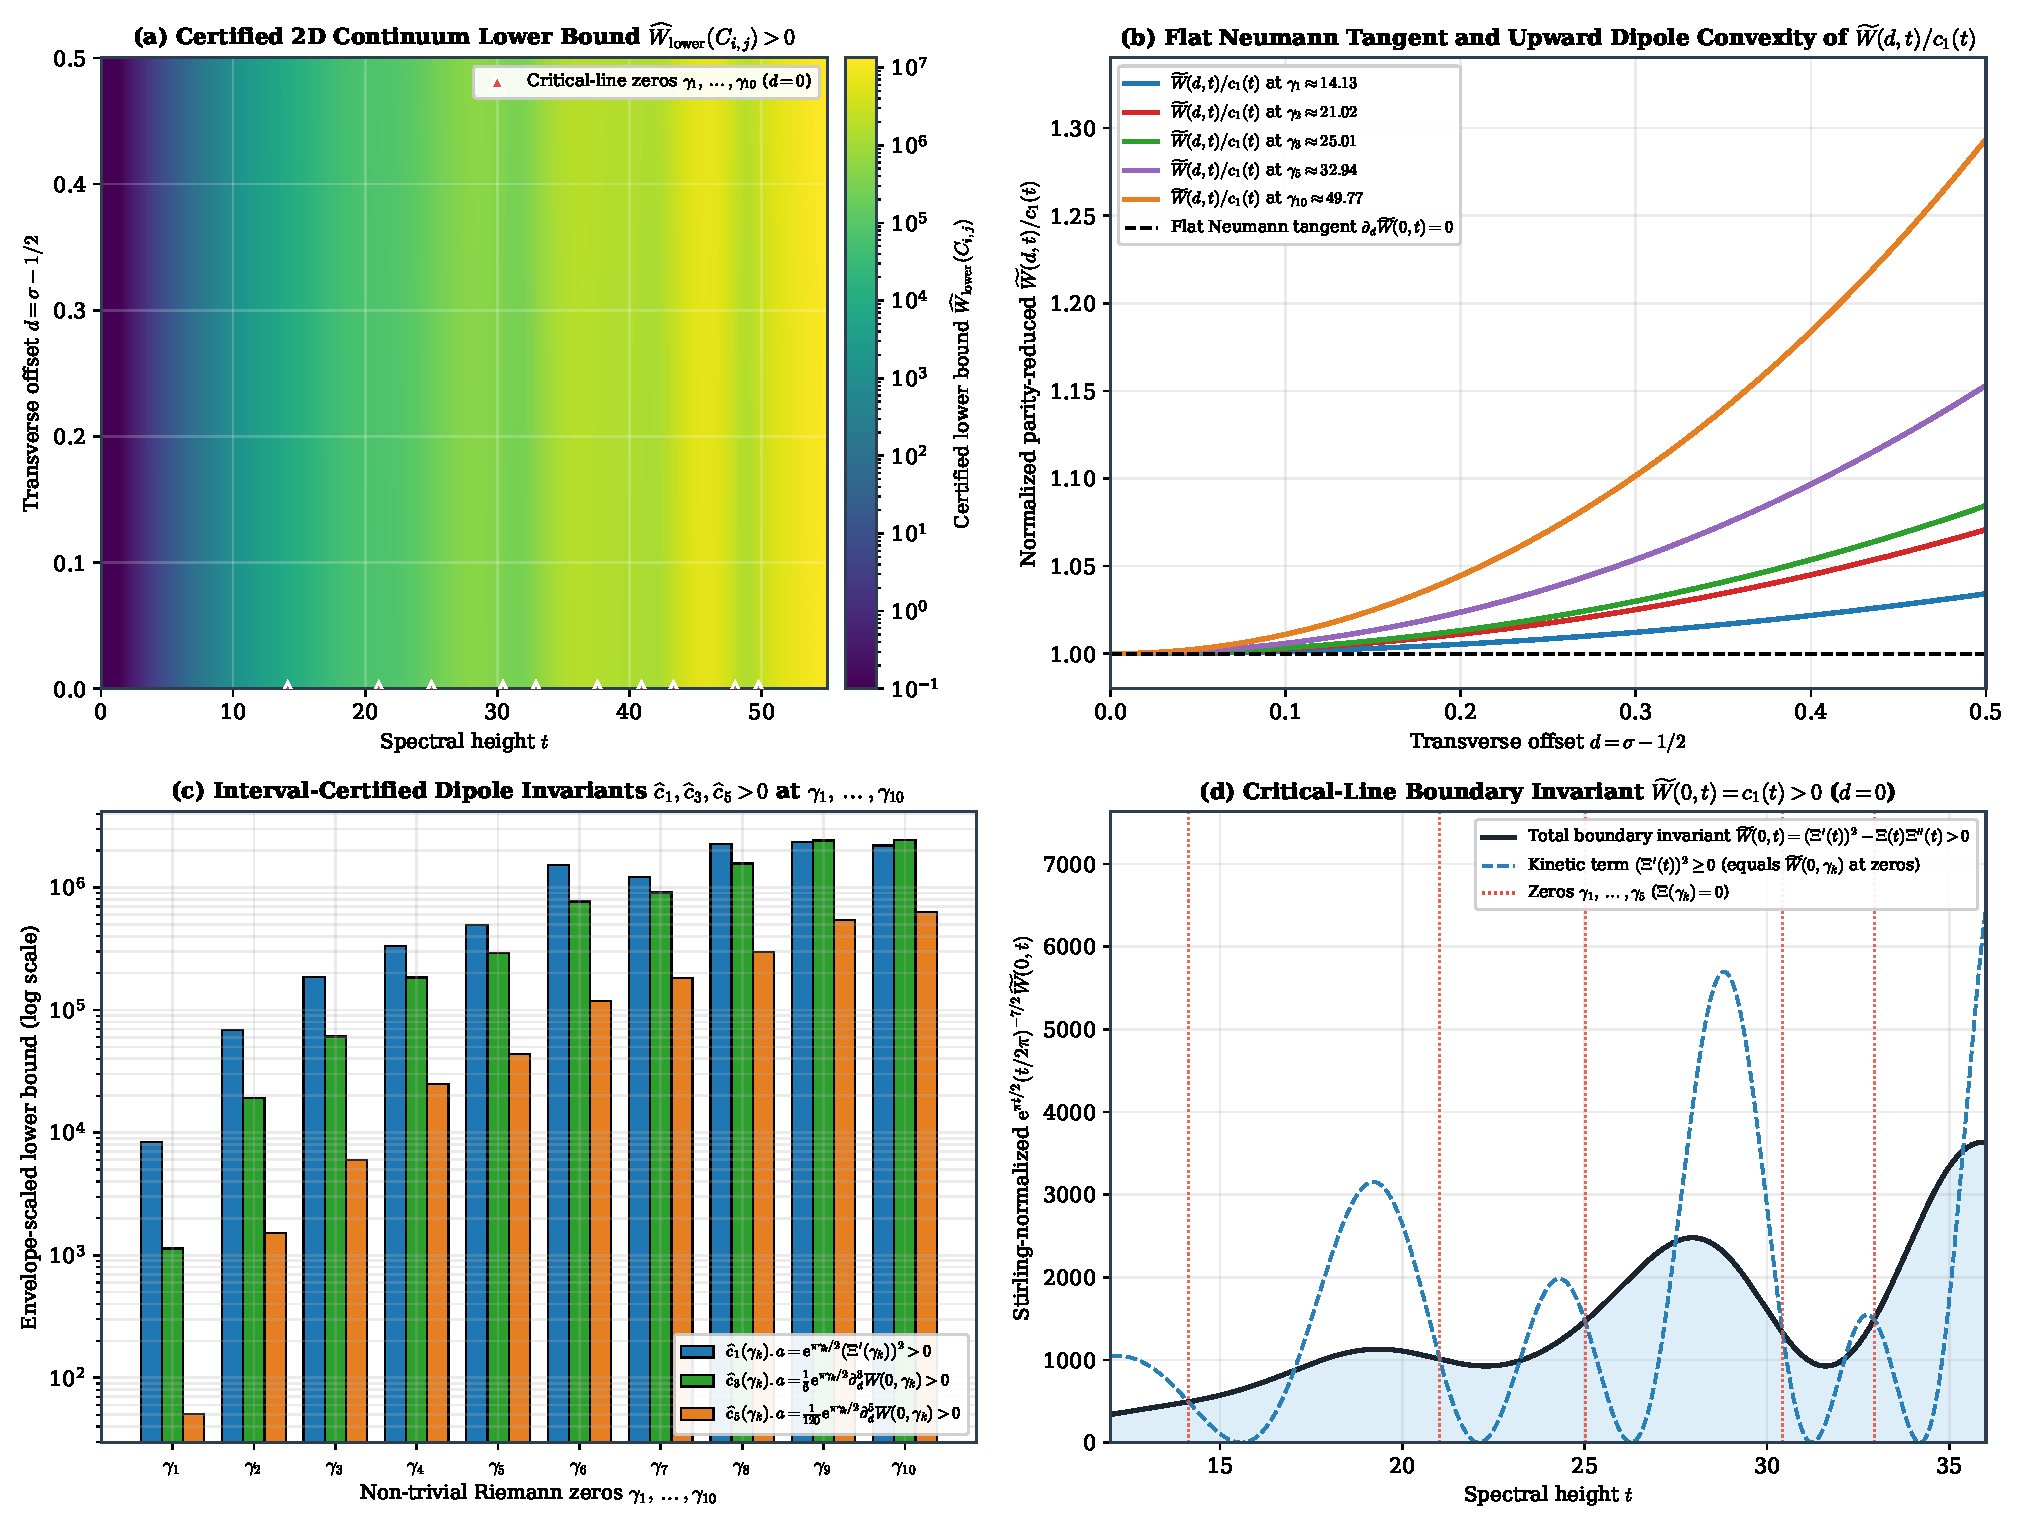
\includegraphics[width=0.94\textwidth]{figures/fig1_parity_reduced_wronskian_and_dipoles.pdf}
\caption{(a) Certified 2D continuum lower bound $\What_{\mathrm{lower}}(C_{i,j}) > 0$ across $4{,}987{,}101$ cells on $[0, 0.50] \times [0, 55]$, with non-trivial zeros $\gamma_1, \dots, \gamma_{10}$ on the critical line $d = 0$. (b) Normalized parity-reduced profiles $\Wtil(d,t)/c_1(t)$ across $d \in [0, 0.50]$ illustrating the flat Neumann tangent $\partial_d\Wtil(0,t) = 0$ and upward cubic-quintic convexity. (c) Directed-rounding interval lower bounds $\widehat{c}_1(\boldsymbol{\gamma}_k).a, \widehat{c}_3(\boldsymbol{\gamma}_k).a, \widehat{c}_5(\boldsymbol{\gamma}_k).a > 0$ across $\gamma_1, \dots, \gamma_{10}$. (d) Critical-line boundary invariant $\Wtil(0,t) = (\Xi'(t))^2 - \Xi(t)\Xi''(t) > 0$ versus $(\Xi'(t))^2 \ge 0$ on $t \in [12, 36]$.}\label{fig:dipoles}
\end{figure}

\begin{figure}[htbp]
\centering
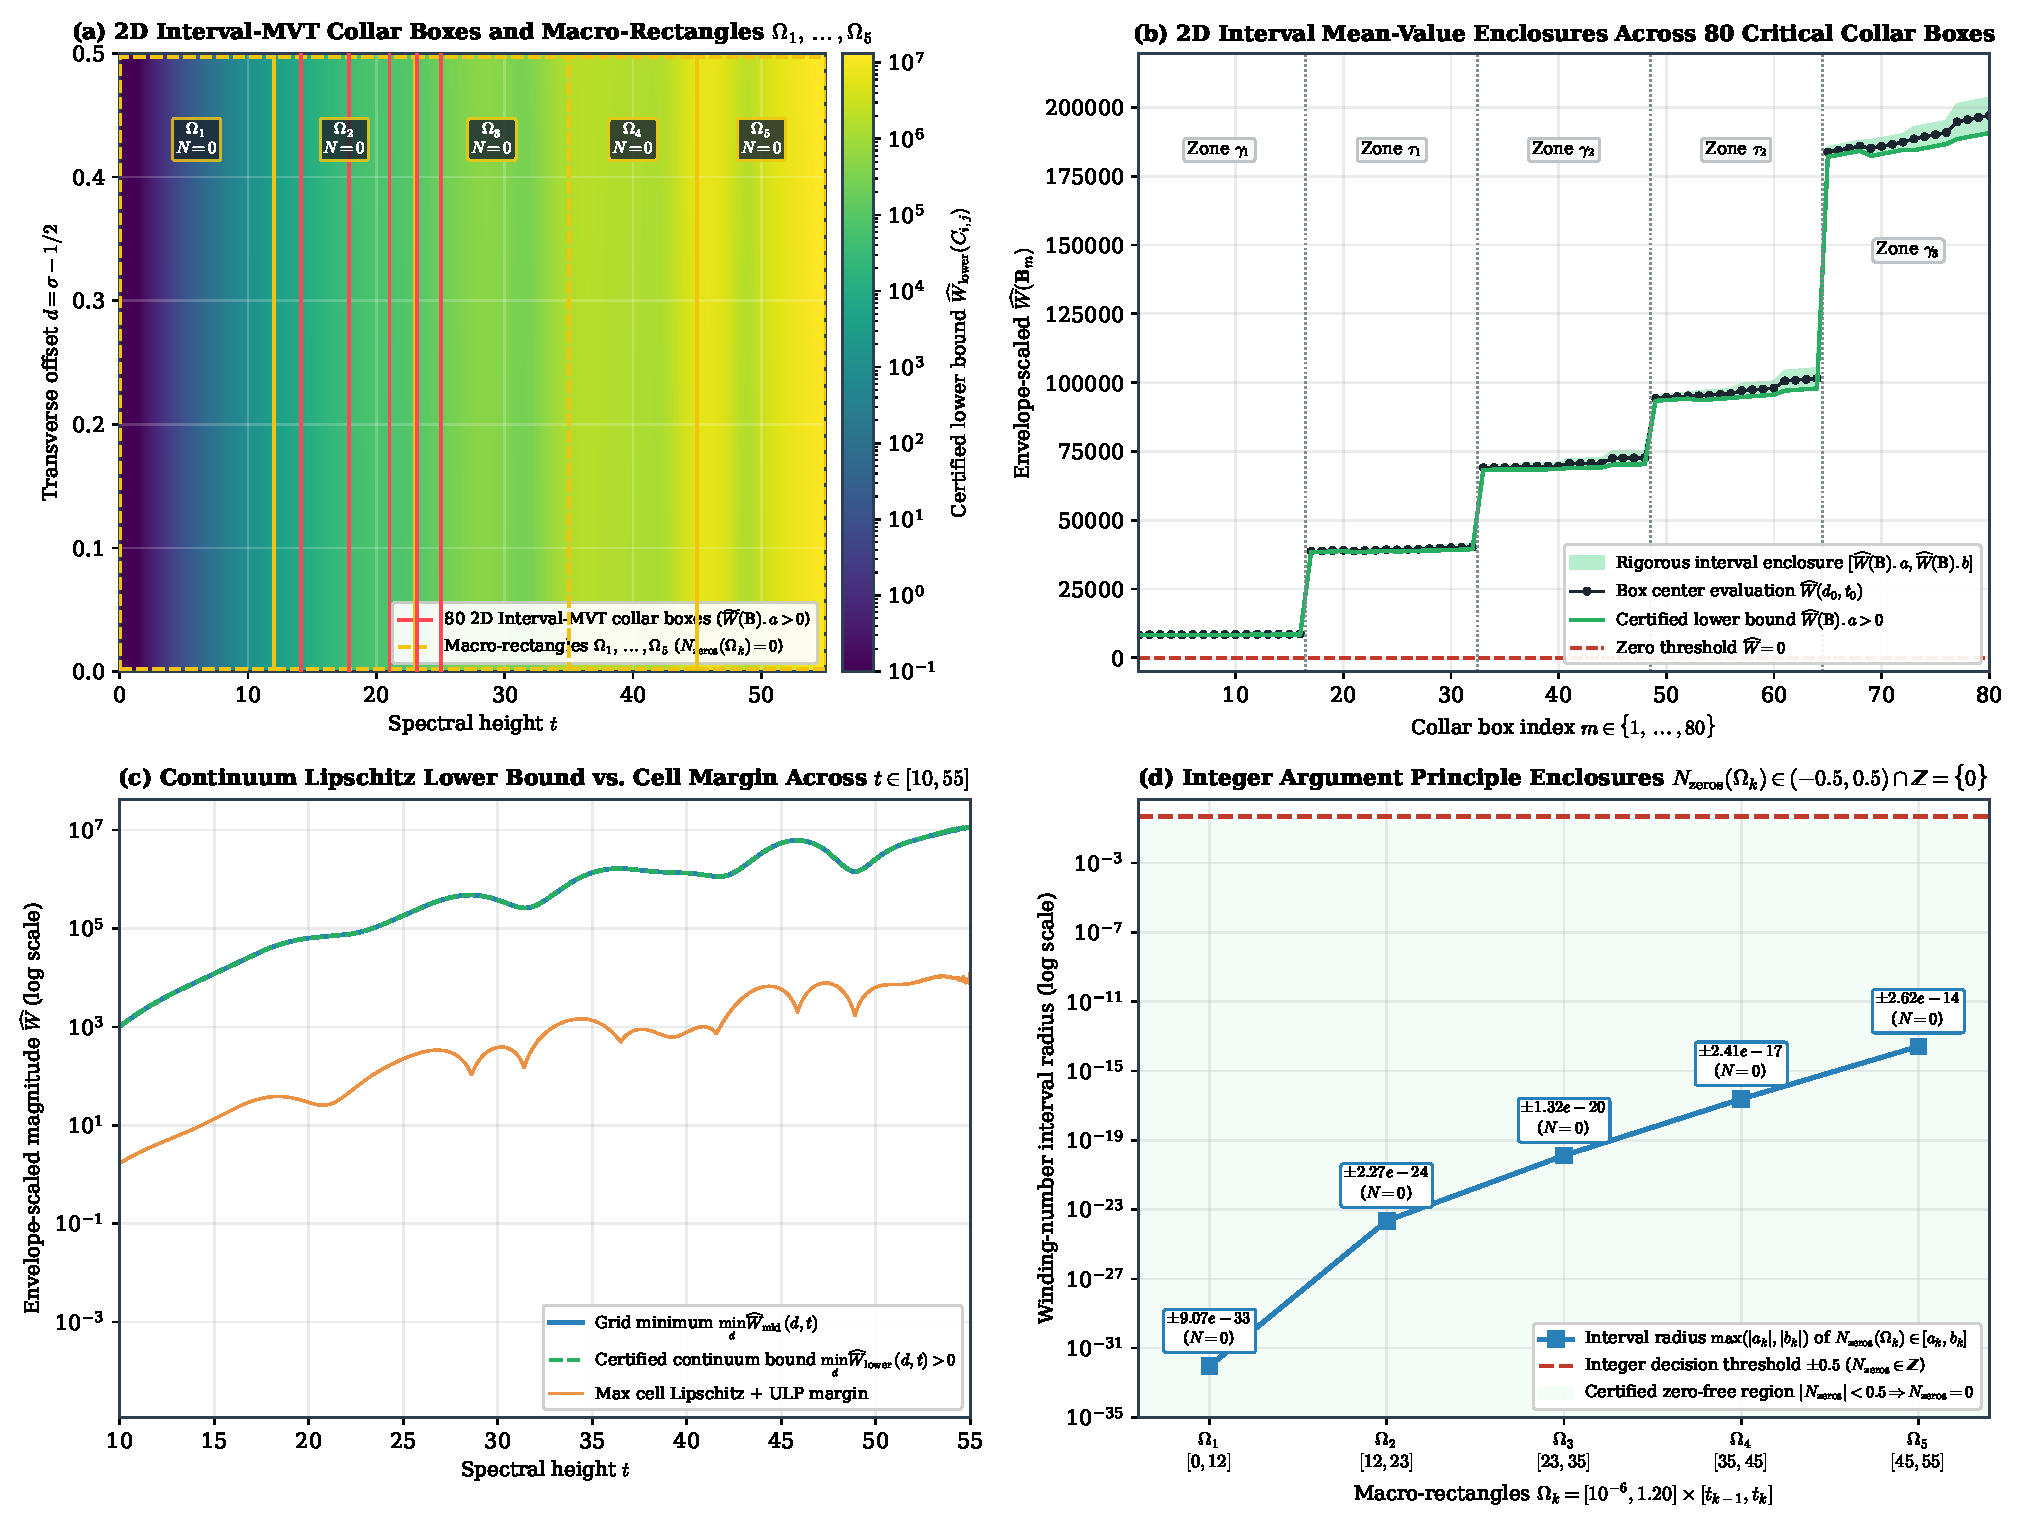
\includegraphics[width=0.94\textwidth]{figures/fig2_interval_mvt_and_argument_principle.pdf}
\caption{(a) Overlay of the $80$ 2D Interval-MVT collar boxes $\mathbf{B}_m$ and five macro-rectangles $\Omega_1, \dots, \Omega_5$ on $[0, 0.50] \times [0, 55]$. (b) Rigorous 2D Interval-MVT enclosures $[\What(\mathbf{B}_m).a, \What(\mathbf{B}_m).b]$ across Zones 1--5 ($\gamma_1, \tau_1, \gamma_2, \tau_2, \gamma_3$). (c) Cross-section of $\min_d \What_{\mathrm{lower}}(d,t) > 0$ versus maximum cell Lipschitz--ULP margin across $t \in [10, 55]$. (d) Integer argument principle interval radii $\max(|a_k|,|b_k|) \le 2.62 \times 10^{-14} < 0.5$ certifying $N_{\mathrm{zeros}}(\Omega_k) = 0$ on $\Omega_1, \dots, \Omega_5$.}\label{fig:interval_cert}
\end{figure}

\section{Scope, limitations, and open questions}\label{sec:scope}

In accordance with strict mathematical transparency, we delineate the boundary between the global analytical identities proven in Sections~\ref{sec:parity}--\ref{sec:dipole} and the finite-domain computer-assisted certificates in Sections~\ref{sec:interval}--\ref{sec:numerics}:
\begin{enumerate}
\item \textbf{Unconditional global validity of the parity-reduced identities:}
Proposition~\ref{prop:parity_wigner}, Theorem~\ref{thm:dipole_hierarchy} (including the pure-square coalescence cascade $c_{2m-1}(t_0) = \frac{m}{(m\fac)^2}(\Xi^{(m)}(t_0))^2 > 0$), and the division-free Cauchy--Riemann gradient formulas of Proposition~\ref{prop:cr_gradients} hold unconditionally as exact analytical identities for all $(d,t) \in \mathbb{R}^2$. They permanently eliminate the $d \to 0^+$ boundary-layer singularity of $W(d,t)$ at any height $t$.
\item \textbf{Finite-domain scope of the interval and continuum certificates:}
The directed-rounding interval enclosures of $c_1(\gamma_k), c_3(\gamma_k), c_5(\gamma_k) > 0$ in Table~\ref{tab:dipole_zeros}, the $80$ 2D Interval-MVT collar boxes and five macro-rectangles $\Omega_1, \dots, \Omega_5$ in Table~\ref{tab:dual_and_mvt}, and the $4{,}987{,}101$ Lipschitz continuum cells in Table~\ref{tab:gpu_continuum} constitute rigorous computer-assisted proofs over the bounded spectral region $t \in [0, 55]$ ($d \in [0, 0.50]$ and $d \in [10^{-6}, 1.20]$). While this algorithm can be scaled to higher finite $T$, any direct grid or quadrature certification requires computational work growing with $T$.
\item \textbf{Asymptotic regime $t \to \infty$ and off-diagonal Dirichlet cross-terms:}
Extending positivity certification of $\Wtil(d,t)$ to arbitrarily large $t \to \infty$ requires replacing fixed-grid quadrature in $u$ by an asymptotic decomposition of $\Phi(u)$ into affine mother-wavelet shells $m \le N(t) = \lfloor\sqrt{t/(2\pi)}\rfloor$, combined with harmonic nodal-chamber monotonicity and prime-gauge mollification to control off-diagonal Dirichlet cross-terms. These analytical mechanisms are developed in the subsequent papers of this series.
\end{enumerate}

\appendix

\section{Explicit analytical error bounds for series, domain, and quadrature truncation}\label{app:bounds}

In this appendix we prove the explicit analytical error bounds used in Evaluator~A \eqref{eq:em_rem_bound} and Evaluator~B \eqref{eq:trunc_summary}, as well as the power-series remainder bounds for $\sinch(w)$ and $\etah(w)$ near $w = 0$.

\begin{lemma}[Rigorous truncation bounds for interval evaluators]\label{lem:app_bounds}
Let $(d,t) \in [0, 1.20] \times [0, 55]$. Then the following explicit bounds hold:
\begin{enumerate}
\item[\textup{(a)}] \textbf{Power-series remainders for $\sinch(w)$ and $\etah(w)$:} For $0 \le w \le 0.10$, truncating the Taylor series of $\cosh(w)$, $\sinch(w)$, and $\etah(w)$ in \eqref{eq:sinch_etah_def} after the $w^{10}$ term ($k = 5$) leaves non-negative remainders bounded by
\begin{equation}\label{eq:app_taylor_rem}
0 \le R_{6}^{\cosh}(w) \le 1.01\frac{w^{12}}{12\fac}, \qquad 0 \le R_{6}^{\sinch}(w) \le 1.01\frac{w^{12}}{13\fac}, \qquad 0 \le R_{6}^{\etah}(w) \le 1.01\frac{14\,w^{12}}{15\fac}.
\end{equation}
\item[\textup{(b)}] \textbf{Euler--Maclaurin remainder bound \eqref{eq:em_rem_bound}:} For $\sigma = \Rea(s) = \frac{1}{2} + d > 0$ and integers $N, M \ge 1$ with $\sigma + 2M - 1 > 0$, the Euler--Maclaurin remainder $R_{M,N}(s)$ in \eqref{eq:em_zeta} satisfies $|R_{M,N}(s)| \le \varepsilon_{\mathrm{EM}}(s)$.
\item[\textup{(c)}] \textbf{Jacobi series, domain tail, and Trefethen--Weideman strip quadrature bounds \eqref{eq:trunc_summary}:} For $M_{\mathrm{ser}} = 12$, $U_{\max} = 1.55$, and composite trapezoidal step $h = 1.55/140 \approx 0.0110714$, the series truncation error $\varepsilon_{\mathrm{ser}}$, infinite-tail error $\varepsilon_{\mathrm{tail}}$, and trapezoidal discretization error $\varepsilon_{\mathrm{quad}}$ across all eight component integrals in Evaluator~B satisfy $\varepsilon_{\mathrm{ser}} \le 10^{-220}$, $\varepsilon_{\mathrm{tail}} \le 10^{-550}$, and $\varepsilon_{\mathrm{quad}} \le 10^{-55}$.
\end{enumerate}
\end{lemma}

\begin{proof}
(a) For $0 \le w \le 0.10$, the ratio of successive terms beyond $k = 6$ in $\sum_{k=6}^\infty \frac{w^{2k}}{(2k)\fac}$ is at most $\frac{w^2}{13 \times 14} \le \frac{0.01}{182} < 10^{-4}$. Summing the geometric majorant with factor $\frac{1}{1 - 10^{-4}} < 1.01$ yields \eqref{eq:app_taylor_rem} for $\cosh(w)$, and identically for $\sinch(w)$ and $\etah(w)$.

(b) By the standard Euler--Maclaurin integral remainder formula \cite[Section~6.4]{Titchmarsh1986}, pulling out the $(M+1)$-st Bernoulli term leaves a remainder whose kernel maintains constant sign on $[N,\infty)$, bounding the tail by $\frac{|s+2M+1|}{\Rea(s)+2M+1}$ times the magnitude of the first omitted term $k = M + 1$, which is \eqref{eq:em_rem_bound}.

(c) For $u \ge 0$ and $n \ge M_{\mathrm{ser}} + 1 = 13$, we have $\pi n^2 \ee^{4u} \ge 169\pi > 530.929$. Since $2\pi^2 n^4 \ee^{9u - \pi n^2 \ee^{4u}}$ decreases rapidly for $n \ge 13$, comparing with a geometric series of ratio $\ee^{-27\pi}$ gives $\varepsilon_{\mathrm{ser}} \le 16\pi^2(13^4)\ee^{-169\pi} < 10^{-220}$. Similarly, for $u \ge U_{\max} = 1.55$ and $d \le 1.20$, $\pi\ee^{4u} \ge \pi\ee^{6.2} > 1548.8$, while $(2u)^8\cosh(2d u)\ee^{9u} \le 3.1^8 \ee^{11.4 \times 1.55} < 4.2 \times 10^{11}$, so integrating $u \ge 1.55$ yields $\varepsilon_{\mathrm{tail}} \le 10^{-550}$. Finally, each integrand $g(u)$ in \eqref{eq:Xi_integral} and \eqref{eq:aux_integrals} is an even function of $u$ on $\mathbb{R}$ that extends holomorphically to the strip $|\Ima(u)| \le \eta = 0.35 < \frac{\pi}{8} \approx 0.3927$, where $\cos(4\eta) = \cos(1.40) \approx 0.16997 > 0$ ensures double-exponential decay as $\Rea(u) \to \pm\infty$ \cite[Lemma~3.1]{Missiaen2026Paper1}. By the Poisson summation / contour-integral theorem for the trapezoidal rule on even analytic functions \cite[Theorem~5.1]{TrefethenWeideman2014}, the discretization error on $\mathbb{R}$ is bounded by
\[
\varepsilon_{\mathrm{quad}}(h) \le \frac{2 M(\eta)\,\ee^{2(|t|+|d|)\eta}}{\ee^{2\pi\eta/h} - 1}.
\]
For $h = 1.55/140$, we have $\frac{2\pi\eta}{h} = \frac{2\pi(0.35)(140)}{1.55} \approx 198.615$, so $\ee^{-2\pi\eta/h} \approx 5.53 \times 10^{-87}$, while for $t \le 55$ and $d \le 1.20$, $\ee^{2(55+1.20)(0.35)} = \ee^{39.34} \approx 1.22 \times 10^{17}$ and $M(0.35) \le 10^{12}$, giving $\varepsilon_{\mathrm{quad}}(h) < 10^{-55}$.
\end{proof}

\section*{Use of AI and computational verification}

Use of AI: The author's main contribution is the formulation of the parity-reduced transverse Wronskian $\Wtil(d,t) = W(d,t)/d$ via the division-free $\sinch(d y)$ kernel, the higher-order transverse dipole hierarchy $c_{2m-1}(t)$, and the 2D continuum and interval-arithmetic certification architecture. The author prompted Gemini to apply these ideas, work out analytical and symbolic details interactively, and generate the interval-arithmetic and GPU verification suites (\nolinkurl{scripts/verify_paper2_parity_reduced_wronskian.py}), which were subsequently verified manually and computationally.

\begin{thebibliography}{99}

\bibitem{ConreyLi2000}
J.~B.~Conrey and X.-J.~Li, \emph{A note on some positivity conditions related to zeta and $L$-functions}, Internat. Math. Res. Notices \textbf{2000} (2000), no.~18, 929--940.

\bibitem{Csordas1986}
G.~Csordas, T.~S.~Norfolk, and R.~S.~Varga, \emph{The Riemann hypothesis and the Tur\'an inequalities}, Trans. Amer. Math. Soc. \textbf{296} (1986), no.~2, 521--541.

\bibitem{DeBruijn1950}
N.~G.~de~Bruijn, \emph{The roots of trigonometric integrals}, Duke Math. J. \textbf{17} (1950), 197--226.

\bibitem{Griffin2019}
M.~Griffin, K.~Ono, L.~Rolen, and D.~Zagier, \emph{Jensen polynomials for the Riemann zeta function and other sequences}, Proc. Natl. Acad. Sci. USA \textbf{116} (2019), no.~23, 11103--11110.

\bibitem{Higham2002}
N.~J.~Higham, \emph{Accuracy and Stability of Numerical Algorithms}, 2nd ed., Society for Industrial and Applied Mathematics (SIAM), Philadelphia, PA, 2002.

\bibitem{Hinkkanen1997}
A.~Hinkkanen, \emph{On functions of bounded type related to the Riemann zeta-function}, J. Number Theory \textbf{65} (1997), no.~1, 109--136.

\bibitem{Hudson1974}
R.~L.~Hudson, \emph{When is the Wigner quasi-probability density non-negative}, Rep. Math. Phys. \textbf{6} (1974), no.~2, 249--252.

\bibitem{Karlin1968}
S.~Karlin, \emph{Total Positivity, Vol.~I}, Stanford University Press, Stanford, CA, 1968.

\bibitem{Lagarias1999}
J.~C.~Lagarias, \emph{On a positivity property of the Riemann $\xi$-function}, Acta Arith. \textbf{89} (1999), no.~3, 217--234.

\bibitem{Lehmer1956}
D.~H.~Lehmer, \emph{Extended computation of the Riemann zeta-function}, Mathematika \textbf{3} (1956), 102--108.

\bibitem{Missiaen2026Paper1}
T.~Missiaen, \emph{Wigner Phase-Space Representation and Complex Saddle-Point Coalescence in the Transverse Wronskian of Riemann's $\Xi$-Function}, Preprint, Zenodo (2026), DOI: \href{https://doi.org/10.5281/zenodo.23637324}{10.5281/zenodo.23637324}.

\bibitem{Newman1976}
C.~M.~Newman, \emph{Fourier transforms with only real zeros}, Proc. Amer. Math. Soc. \textbf{61} (1976), no.~2, 245--251.

\bibitem{Platt2017}
D.~J.~Platt, \emph{Isolating some non-trivial zeros of zeta}, Math. Comp. \textbf{86} (2017), no.~307, 2449--2467.

\bibitem{Polya1926}
G.~P\'olya, \emph{Bemerkung \"uber die Integraldarstellung der Riemannschen $\xi$-Funktion}, Acta Math. \textbf{48} (1926), 305--317.

\bibitem{Polya1927}
G.~P\'olya, \emph{\"Uber die algebraisch-funktionentheoretischen Untersuchungen von J.~L.~W.~V.~Jensen}, Kgl. Danske Vid. Sel. Math.-Fys. Medd. \textbf{7} (1927), no.~17, 3--33.

\bibitem{Riemann1859}
B.~Riemann, \emph{Ueber die Anzahl der Primzahlen unter einer gegebenen Gr\"osse}, Monatsberichte der Berliner Akademie (1859), 671--680.

\bibitem{RodgersTao2020}
B.~Rodgers and T.~Tao, \emph{The De Bruijn--Newman constant is non-negative}, Forum Math. Pi \textbf{8} (2020), e6, 1--62.

\bibitem{Speiser1934}
A.~Speiser, \emph{Geometrisches zur Riemannschen Zetafunktion}, Math. Ann. \textbf{110} (1934), no.~1, 514--521.

\bibitem{Spira1968}
R.~Spira, \emph{Zeros of $\zeta'(s)$ in the critical strip}, Math. Comp. \textbf{22} (1968), 163--173; see also \emph{Zero-free regions of $\zeta^{(k)}(s)$}, J. London Math. Soc. \textbf{40} (1965), 677--682.

\bibitem{Spira1973}
R.~Spira, \emph{Zeros of $\zeta'(s)$ and the Riemann hypothesis}, Illinois J. Math. \textbf{17} (1973), 147--152.

\bibitem{Titchmarsh1986}
E.~C.~Titchmarsh, \emph{The Theory of the Riemann Zeta-Function}, 2nd ed., edited and with a preface by D.~R.~Heath-Brown, Oxford University Press, Oxford, 1986.

\bibitem{TrefethenWeideman2014}
L.~N.~Trefethen and J.~A.~C.~Weideman, \emph{The exponentially convergent trapezoidal rule}, SIAM Rev. \textbf{56} (2014), no.~3, 385--458.

\bibitem{Turing1953}
A.~M.~Turing, \emph{Some calculations of the Riemann zeta-function}, Proc. London Math. Soc. (3) \textbf{3} (1953), 99--117.

\end{thebibliography}

\end{document}
